\chapter{Metrical Facility Location algorithms}

\section{Problem description}

Problem instance consists of a full bipartite graph $G = (F \cup C, F \times
C)$, where elements of $F$ are called \emph{facilities} and those of $C$ are
called \emph{cities}, $o : F \to \mathbb{R}$ being a cost function of opening
single facility and $c : F \times C \to \mathbb{R}$ being a cost function of
connecting facility with a city. The connection costs satisfy triangle
inequality.

The problem is to find a subset of facilities $O \subset F$ to be opened and an
assignment of cities to opened facilities $a : C \to O$ in such a way that the
total cost $\sum_{f \in O} o(f) + \sum_{c \in C} c(a(c), c)$ is minimized.

\section{Primal-dual schema 3-apx}
We have created efficient implementation of combinatoric approximation
algorithm for the problem as a reference point for other discussed methods. The
algorithm achieves a constant approximation factor of 3 and runs in $\Oh(|F||C|
\log(|F||C|))$ time. It operates in primal-dual fashion trying to find feasible
solution for dual problem with possibly the biggest cost. Detailed description
can be found in \cite{Vazirani}.

We have introduced a slight modification to original algorithm due to Jain and
Vasirani. Once the set of opened facilities is determined as in original
algorithm we create optimal assignment in $\Oh(|F||C|)$ time by assigning each
city to the closest facility. The assignment presented in original paper is
useful for estimating approximation factor of the algorithm though.

\section{Local Search 3-apx}

Local search with the following properties
guarantees\footnote{\url{http://www.cs.ucla.edu/~awm/papers/lsearch.ps}}
3-apx at local optimum:
\begin{itemize}
\item Search space consists of all subsets of facilities.
\item Fitness function is the same as in problem statement.
\item Valid step is of one of the forms:
	\begin{itemize}
	\item insert one facility to the set
	\item delete one facility from the set
	\item swap one facility from the set with one from outside the set.
	\end{itemize}
\end{itemize}

We have implemented 2 variants of Walkers (see: Local Search Framework design)
for this algorithm:
\begin{itemize}
\item RandomStepWalker: take a random valid step and calculate fitness: $\Oh(|F||C|)$ per iteration
\item BestStepWalker: find the fittest step among the valid ones: $\Oh(|F|(|F|+|C|))$ per iteration
\end{itemize}

In both cases, time of single iteration is proportional to the problem
instance size. It is therefore necessary to start the local search from
the solution relatively close (in the topology described) to the local
optimum. Intuitively the optimal solution will consist of a small number
of facilities (especially for test cases with uniformly distributed facilities and cities),
therefore the initial solution has been set to an empty set.

\section{Monte Carlo Tree Search}

We will refer to the concepts and definitions introduced in MCTS design
chapter. Let us remind that the only domain-dependent concepts in our MCTS
framework are Move and State and the former is completely dependent on the
latter.

Because MCTS involves selecting decisions step by step we decided to transform our
standard Facility Location problem into Online Facility Location problem.
\begin{itemize}
\item State is a vector of already opened facilities and an ordering in which
next facilities will be processed.
\item Initial State is empty vector (opened facilities) and a permutation
of $1,2,\dots, |F|$ (ordering).
\item Move represent a choice if facility should be opened in given point or not.
\item Terminal state is when all facilities have been processed (each one is
considered only once).
\item Fitness of terminal State is equal to sum of openning costs and connection costs.
\item Fitness estimate is calculated using Adam Meyerson's algorithm\footnote{\url{http://www.cs.ucla.edu/~awm/papers/ofl.pdf}}
which is constant competitive for randomized input.
\end{itemize}

\section{Random Search}

As an additional benchmark for evaluating algorithms' performance, we've implemented
random search, which simply samples solution space at random. Solutions are drawn as follows:
\begin{itemize}
\item draw with uniform distribution the solution size $n \in \{1..|F|\}$.
\item draw $n$ times a facility with uniform distribution.
\item solution is the set of facilities from the previous point.
\end{itemize}

We've empirically shown for the benchmark problem instances, that the near optimal
solutions are small sets. This drawing algorithm is flexible enough to take it
into consideration.

\section{Benchmarks}
To evaluate the algorithms quality we have used UflLib\footnote{\url{http://www.mpi-inf.mpg.de/departments/d1/projects/benchmarks/UflLib/Euklid.html}}
and our "clustered tests". The need for "clustered tests" raised from observation that
uniform distribution is not natural for many real-world situation like city placements
e.g. normally cities are "clustered" around natural resources.

\subsection{Clustered tests}

Clustered tests are euclidian plane tests.
All facilities and cities are placed in the $[0,1]^2$ square.
Test generation begins with drawing the clusters.
Cluster is a rectangle, whose dimensions are drawn uniformly from the test case specific ranges (usually from $.1$ to $.4$).
Cluster positions are drawn so that the whole cluster fits into the unit square.
Number of clusters is test specific (from 10 to 30). Clusters can overlap.
Once the clusters are determined, facilities and cities are being drawn (their number is test specific; usually about ~100 facilities and ~1000 cities).
For each facility/city the cluster it will fall in is drawn with uniform probability.
The actual position is selected with uniform probability from the cluster rectangle.
Sample tests are depicted on figures \ref{FLClustered/test2.txt}-\ref{FLClustered/test4.txt}.

\pgfsetplotmarksize{2pt}
\begin{figure}
	\centering
 \caption{\label{FLClustered/test0.txt}FLClustered/test0.txt},
	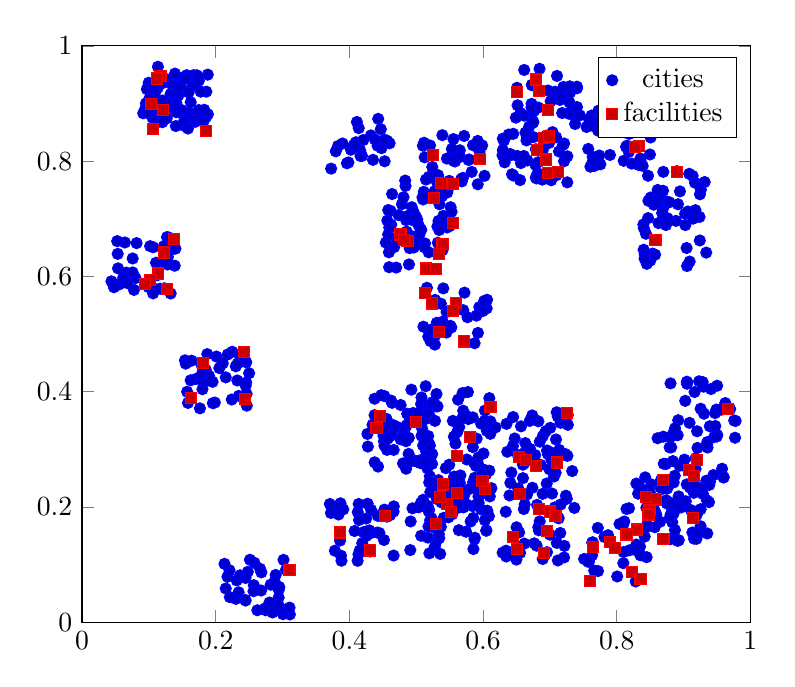
\begin{tikzpicture}
	\begin{axis}[
		width=0.7\textwidth,
		scale only axis,
		xmin=0,xmax=1,ymin=0,ymax=1,
		only marks]
		\addplot coordinates {
			(0.461584, 0.713681)
			(0.950261, 0.41024)
			(0.245626, 0.416019)
			(0.462603, 0.68957)
			(0.519238, 0.195222)
			(0.0757554, 0.631054)
			(0.460862, 0.185712)
			(0.511756, 0.831811)
			(0.535942, 0.751933)
			(0.590437, 0.318553)
			(0.977946, 0.349284)
			(0.561501, 0.330219)
			(0.88514, 0.188477)
			(0.602232, 0.774414)
			(0.681677, 0.778896)
			(0.904962, 0.417286)
			(0.535449, 0.765505)
			(0.0662904, 0.606478)
			(0.612545, 0.232577)
			(0.536942, 0.165522)
			(0.539014, 0.698584)
			(0.605814, 0.332067)
			(0.565291, 0.241689)
			(0.678875, 0.77133)
			(0.721783, 0.13245)
			(0.165231, 0.930406)
			(0.725497, 0.922153)
			(0.16701, 0.949027)
			(0.452254, 0.39244)
			(0.466083, 0.191946)
			(0.634741, 0.114014)
			(0.891683, 0.725114)
			(0.8806, 0.414363)
			(0.902734, 0.689014)
			(0.688672, 0.767825)
			(0.457199, 0.19312)
			(0.38983, 0.830546)
			(0.230255, 0.0405551)
			(0.540533, 0.579163)
			(0.935471, 0.154029)
			(0.875036, 0.206298)
			(0.762374, 0.879031)
			(0.733431, 0.262286)
			(0.919495, 0.185889)
			(0.610162, 0.218287)
			(0.491141, 0.125153)
			(0.695355, 0.24068)
			(0.662345, 0.204428)
			(0.844769, 0.112919)
			(0.5715, 0.219418)
			(0.718518, 0.354371)
			(0.0538975, 0.613879)
			(0.141204, 0.90102)
			(0.800767, 0.0793937)
			(0.507892, 0.281791)
			(0.700563, 0.337246)
			(0.600647, 0.292762)
			(0.217635, 0.0789491)
			(0.535883, 0.118534)
			(0.949185, 0.368901)
			(0.55497, 0.195589)
			(0.740532, 0.926323)
			(0.530479, 0.765113)
			(0.230081, 0.443999)
			(0.153108, 0.861152)
			(0.512723, 0.806536)
			(0.654024, 0.155863)
			(0.188123, 0.949962)
			(0.608766, 0.183867)
			(0.527741, 0.130911)
			(0.661829, 0.136419)
			(0.594481, 0.546692)
			(0.602943, 0.26385)
			(0.888672, 0.696302)
			(0.218038, 0.464535)
			(0.689344, 0.10974)
			(0.60544, 0.544424)
			(0.829446, 0.134892)
			(0.231443, 0.0726643)
			(0.551505, 0.719979)
			(0.721303, 0.830557)
			(0.650906, 0.927116)
			(0.642332, 0.810737)
			(0.772027, 0.0888079)
			(0.274789, 0.0208715)
			(0.631156, 0.835453)
			(0.917979, 0.265974)
			(0.84885, 0.871267)
			(0.875444, 0.231974)
			(0.665058, 0.835887)
			(0.289739, 0.0820553)
			(0.471739, 0.338643)
			(0.597299, 0.195695)
			(0.649963, 0.108654)
			(0.482099, 0.332692)
			(0.162563, 0.419777)
			(0.245752, 0.450941)
			(0.712377, 0.181791)
			(0.853597, 0.639525)
			(0.257062, 0.0642846)
			(0.78166, 0.14786)
			(0.416192, 0.818516)
			(0.142586, 0.920643)
			(0.840338, 0.646178)
			(0.431244, 0.154147)
			(0.442272, 0.826705)
			(0.549387, 0.273279)
			(0.584604, 0.201418)
			(0.421008, 0.156218)
			(0.548403, 0.753739)
			(0.568243, 0.224429)
			(0.879571, 0.143776)
			(0.669883, 0.349265)
			(0.581487, 0.174796)
			(0.201079, 0.460929)
			(0.731097, 0.881586)
			(0.102377, 0.888931)
			(0.896349, 0.199155)
			(0.511358, 0.746695)
			(0.516859, 0.202209)
			(0.242756, 0.454301)
			(0.0996819, 0.581415)
			(0.945843, 0.321448)
			(0.869185, 0.717422)
			(0.514611, 0.278196)
			(0.950586, 0.324732)
			(0.147988, 0.929311)
			(0.0800058, 0.597041)
			(0.169522, 0.868138)
			(0.737777, 0.864311)
			(0.144185, 0.914114)
			(0.601265, 0.264097)
			(0.818922, 0.124762)
			(0.26231, 0.0208061)
			(0.427703, 0.30476)
			(0.520883, 0.176977)
			(0.846857, 0.77457)
			(0.548192, 0.216499)
			(0.0641223, 0.658804)
			(0.947182, 0.362977)
			(0.138485, 0.887881)
			(0.176373, 0.371064)
			(0.174732, 0.939457)
			(0.136953, 0.942888)
			(0.923942, 0.703139)
			(0.372398, 0.189621)
			(0.913971, 0.705291)
			(0.887121, 0.160038)
			(0.944758, 0.255353)
			(0.757431, 0.821088)
			(0.640872, 0.24176)
			(0.850311, 0.627418)
			(0.709902, 0.775529)
			(0.500999, 0.695805)
			(0.525901, 0.379984)
			(0.517382, 0.146865)
			(0.892706, 0.218335)
			(0.555999, 0.247286)
			(0.48645, 0.361778)
			(0.555738, 0.838189)
			(0.554047, 0.239191)
			(0.891996, 0.350441)
			(0.668977, 0.85958)
			(0.563699, 0.198981)
			(0.531058, 0.213747)
			(0.491697, 0.670444)
			(0.451794, 0.142674)
			(0.185596, 0.876639)
			(0.880737, 0.186859)
			(0.593084, 0.229618)
			(0.555163, 0.233825)
			(0.549401, 0.765658)
			(0.170331, 0.422032)
			(0.833301, 0.236202)
			(0.812258, 0.849888)
			(0.426999, 0.326693)
			(0.127131, 0.668167)
			(0.859112, 0.187162)
			(0.570268, 0.366988)
			(0.913605, 0.774347)
			(0.64604, 0.11707)
			(0.520412, 0.253276)
			(0.763196, 0.116221)
			(0.774011, 0.809672)
			(0.106464, 0.650542)
			(0.55257, 0.511386)
			(0.529141, 0.222465)
			(0.63453, 0.124202)
			(0.925608, 0.196108)
			(0.578194, 0.802099)
			(0.451738, 0.314116)
			(0.584755, 0.303848)
			(0.150492, 0.882225)
			(0.842619, 0.251313)
			(0.187853, 0.425613)
			(0.110453, 0.923853)
			(0.456171, 0.183139)
			(0.841904, 0.148567)
			(0.31098, 0.0135467)
			(0.656051, 0.883384)
			(0.441774, 0.155577)
			(0.442882, 0.270042)
			(0.412579, 0.190942)
			(0.585375, 0.316535)
			(0.470859, 0.664333)
			(0.430003, 0.159317)
			(0.51488, 0.296272)
			(0.837466, 0.794463)
			(0.533332, 0.246448)
			(0.533422, 0.696148)
			(0.480262, 0.275586)
			(0.703922, 0.850239)
			(0.716017, 0.346012)
			(0.53005, 0.139922)
			(0.0776831, 0.576608)
			(0.585627, 0.126941)
			(0.736609, 0.198312)
			(0.430953, 0.122784)
			(0.182839, 0.889009)
			(0.67838, 0.793512)
			(0.565195, 0.818779)
			(0.670337, 0.300848)
			(0.464705, 0.330494)
			(0.562265, 0.209657)
			(0.818215, 0.815916)
			(0.829416, 0.240581)
			(0.108436, 0.578656)
			(0.869339, 0.748449)
			(0.713208, 0.180333)
			(0.710364, 0.137702)
			(0.661683, 0.293498)
			(0.60444, 0.256567)
			(0.41361, 0.117683)
			(0.120454, 0.626282)
			(0.46057, 0.322619)
			(0.810484, 0.800476)
			(0.519348, 0.360176)
			(0.702881, 0.293845)
			(0.215035, 0.424816)
			(0.855378, 0.72442)
			(0.116043, 0.868568)
			(0.754919, 0.859192)
			(0.849725, 0.811462)
			(0.413991, 0.857179)
			(0.527974, 0.481636)
			(0.846993, 0.701093)
			(0.920282, 0.33129)
			(0.916555, 0.399389)
			(0.221164, 0.0435336)
			(0.559552, 0.806365)
			(0.78804, 0.878678)
			(0.938098, 0.208371)
			(0.402293, 0.819733)
			(0.121044, 0.935517)
			(0.539677, 0.52152)
			(0.939284, 0.340023)
			(0.647408, 0.318803)
			(0.592921, 0.273362)
			(0.832759, 0.793333)
			(0.71068, 0.94777)
			(0.470083, 0.61527)
			(0.510658, 0.278225)
			(0.90458, 0.649246)
			(0.789922, 0.810639)
			(0.977084, 0.32011)
			(0.870371, 0.275018)
			(0.099691, 0.935797)
			(0.122377, 0.652317)
			(0.220663, 0.0901681)
			(0.568262, 0.764788)
			(0.234384, 0.0519417)
			(0.673623, 0.358743)
			(0.709136, 0.317122)
			(0.869763, 0.321924)
			(0.456844, 0.696815)
			(0.106052, 0.920878)
			(0.510372, 0.73344)
			(0.640542, 0.812309)
			(0.915345, 0.224497)
			(0.490171, 0.649055)
			(0.530005, 0.233668)
			(0.524373, 0.24385)
			(0.934128, 0.245472)
			(0.56616, 0.254745)
			(0.684871, 0.313213)
			(0.102298, 0.893513)
			(0.713635, 0.816745)
			(0.673428, 0.931533)
			(0.883449, 0.32316)
			(0.571725, 0.843636)
			(0.723141, 0.291802)
			(0.506188, 0.276189)
			(0.602787, 0.34976)
			(0.949482, 0.322071)
			(0.569969, 0.770939)
			(0.182875, 0.878386)
			(0.577889, 0.352456)
			(0.72123, 0.799782)
			(0.661837, 0.276076)
			(0.213173, 0.101288)
			(0.205442, 0.440857)
			(0.913195, 0.155698)
			(0.131483, 0.897276)
			(0.236477, 0.0814496)
			(0.510335, 0.212381)
			(0.594658, 0.816779)
			(0.9171, 0.76255)
			(0.924553, 0.742455)
			(0.90896, 0.345882)
			(0.497007, 0.28076)
			(0.727628, 0.882637)
			(0.478607, 0.725362)
			(0.452405, 0.195359)
			(0.113304, 0.870256)
			(0.868471, 0.231479)
			(0.138722, 0.898761)
			(0.962457, 0.380231)
			(0.61103, 0.34848)
			(0.935921, 0.303089)
			(0.145403, 0.886451)
			(0.676316, 0.887108)
			(0.593202, 0.218424)
			(0.501516, 0.69872)
			(0.0440042, 0.591452)
			(0.889984, 0.782411)
			(0.569421, 0.397576)
			(0.905277, 0.617963)
			(0.154059, 0.454345)
			(0.599703, 0.539945)
			(0.185946, 0.920425)
			(0.665738, 0.841404)
			(0.718407, 0.883397)
			(0.676548, 0.136881)
			(0.527462, 0.743706)
			(0.498819, 0.700761)
			(0.550225, 0.687454)
			(0.672922, 0.871957)
			(0.879758, 0.321437)
			(0.708634, 0.259456)
			(0.606451, 0.193408)
			(0.484998, 0.697537)
			(0.603365, 0.2264)
			(0.396355, 0.796216)
			(0.606011, 0.559433)
			(0.740513, 0.929171)
			(0.673902, 0.233288)
			(0.684807, 0.175079)
			(0.672964, 0.932297)
			(0.4595, 0.615947)
			(0.105737, 0.887555)
			(0.773684, 0.868127)
			(0.84197, 0.638358)
			(0.763309, 0.138326)
			(0.56734, 0.768822)
			(0.850778, 0.221919)
			(0.730616, 0.919563)
			(0.489166, 0.620736)
			(0.854632, 0.189504)
			(0.83544, 0.804373)
			(0.300623, 0.0140221)
			(0.601579, 0.557201)
			(0.14038, 0.860842)
			(0.15951, 0.884254)
			(0.185161, 0.437789)
			(0.682703, 0.164807)
			(0.682857, 0.348645)
			(0.758501, 0.872953)
			(0.132454, 0.916179)
			(0.152442, 0.868324)
			(0.144886, 0.917381)
			(0.684539, 0.960107)
			(0.839924, 0.690014)
			(0.789924, 0.884287)
			(0.629333, 0.120699)
			(0.158485, 0.856539)
			(0.645026, 0.355996)
			(0.282214, 0.0651473)
			(0.15519, 0.448634)
			(0.809552, 0.168642)
			(0.268332, 0.0865295)
			(0.593292, 0.206436)
			(0.702697, 0.28115)
			(0.598766, 0.827144)
			(0.126748, 0.874231)
			(0.843869, 0.865574)
			(0.182163, 0.4204)
			(0.494618, 0.69757)
			(0.123446, 0.941559)
			(0.813881, 0.88447)
			(0.902273, 0.708514)
			(0.719686, 0.347121)
			(0.740564, 0.893786)
			(0.670772, 0.284047)
			(0.519727, 0.119549)
			(0.832061, 0.223061)
			(0.589273, 0.271358)
			(0.892895, 0.142287)
			(0.651671, 0.128735)
			(0.418914, 0.808973)
			(0.462414, 0.32651)
			(0.680189, 0.132851)
			(0.54598, 0.804388)
			(0.586383, 0.27706)
			(0.267985, 0.0550261)
			(0.810265, 0.121762)
			(0.132607, 0.570309)
			(0.928601, 0.416706)
			(0.850836, 0.736857)
			(0.463897, 0.742852)
			(0.386705, 0.206308)
			(0.523404, 0.165867)
			(0.682565, 0.892908)
			(0.541218, 0.181096)
			(0.195305, 0.417125)
			(0.510794, 0.512715)
			(0.652673, 0.232063)
			(0.492762, 0.403499)
			(0.868027, 0.709935)
			(0.383023, 0.826141)
			(0.629123, 0.810138)
			(0.929899, 0.408657)
			(0.452493, 0.306338)
			(0.177634, 0.920494)
			(0.548449, 0.182141)
			(0.933972, 0.641224)
			(0.758668, 0.106013)
			(0.713921, 0.298918)
			(0.294191, 0.0427942)
			(0.867351, 0.733986)
			(0.518899, 0.772542)
			(0.558099, 0.799318)
			(0.906485, 0.712569)
			(0.876119, 0.700825)
			(0.58732, 0.144123)
			(0.541588, 0.209045)
			(0.587679, 0.146596)
			(0.838881, 0.791637)
			(0.585214, 0.242989)
			(0.659632, 0.273346)
			(0.38387, 0.186865)
			(0.0756957, 0.606867)
			(0.0816551, 0.657722)
			(0.24288, 0.457487)
			(0.779023, 0.860114)
			(0.556423, 0.321865)
			(0.512623, 0.27404)
			(0.130275, 0.667344)
			(0.407444, 0.824867)
			(0.116977, 0.578619)
			(0.763052, 0.861704)
			(0.450989, 0.324351)
			(0.645361, 0.774953)
			(0.894661, 0.747452)
			(0.4857, 0.677649)
			(0.721279, 0.112437)
			(0.519229, 0.309837)
			(0.136501, 0.64787)
			(0.12942, 0.903449)
			(0.513067, 0.279576)
			(0.273838, 0.0239683)
			(0.106772, 0.902312)
			(0.677954, 0.290039)
			(0.535294, 0.647412)
			(0.53449, 0.145959)
			(0.689458, 0.322914)
			(0.120162, 0.867553)
			(0.818817, 0.82068)
			(0.675217, 0.868261)
			(0.195743, 0.380046)
			(0.553365, 0.821013)
			(0.671861, 0.880781)
			(0.95975, 0.251023)
			(0.378345, 0.124141)
			(0.540286, 0.65275)
			(0.105304, 0.875258)
			(0.59288, 0.28561)
			(0.869823, 0.701642)
			(0.720416, 0.34895)
			(0.524189, 0.38155)
			(0.139729, 0.648086)
			(0.958992, 0.370066)
			(0.909189, 0.625718)
			(0.493339, 0.720026)
			(0.507899, 0.389959)
			(0.43233, 0.844579)
			(0.288096, 0.07084)
			(0.957685, 0.36907)
			(0.629635, 0.838962)
			(0.925604, 0.370369)
			(0.412368, 0.106584)
			(0.93506, 0.211421)
			(0.549961, 0.698137)
			(0.210574, 0.449158)
			(0.925556, 0.166493)
			(0.458153, 0.715064)
			(0.298421, 0.0229525)
			(0.9356, 0.312546)
			(0.437792, 0.387755)
			(0.65664, 0.796553)
			(0.551031, 0.514272)
			(0.564411, 0.338602)
			(0.496206, 0.711205)
			(0.498033, 0.702863)
			(0.891025, 0.141244)
			(0.577425, 0.399354)
			(0.531826, 0.159716)
			(0.514668, 0.767969)
			(0.822447, 0.795624)
			(0.878471, 0.204072)
			(0.661373, 0.878826)
			(0.710206, 0.364212)
			(0.503371, 0.199324)
			(0.121435, 0.870812)
			(0.585051, 0.827537)
			(0.639562, 0.219953)
			(0.481047, 0.737292)
			(0.701178, 0.903769)
			(0.68633, 0.272946)
			(0.574562, 0.35834)
			(0.537817, 0.207908)
			(0.65681, 0.33983)
			(0.618673, 0.337975)
			(0.697244, 0.922381)
			(0.444937, 0.154695)
			(0.666361, 0.8011)
			(0.527624, 0.747706)
			(0.0956603, 0.900032)
			(0.644858, 0.306029)
			(0.602862, 0.367253)
			(0.957675, 0.266285)
			(0.156534, 0.948973)
			(0.862553, 0.692511)
			(0.54522, 0.502581)
			(0.866234, 0.246501)
			(0.829137, 0.12474)
			(0.78305, 0.862774)
			(0.726945, 0.342534)
			(0.834916, 0.131059)
			(0.507088, 0.207139)
			(0.875407, 0.729624)
			(0.908516, 0.777913)
			(0.39086, 0.195843)
			(0.244873, 0.410513)
			(0.51217, 0.27623)
			(0.502069, 0.278091)
			(0.787094, 0.15095)
			(0.0533604, 0.639051)
			(0.0526267, 0.661116)
			(0.510053, 0.826723)
			(0.507325, 0.378668)
			(0.909585, 0.23364)
			(0.508879, 0.33601)
			(0.187422, 0.465166)
			(0.873752, 0.274495)
			(0.256606, 0.0539277)
			(0.518525, 0.192752)
			(0.554813, 0.34933)
			(0.38248, 0.201778)
			(0.140931, 0.884799)
			(0.939595, 0.243968)
			(0.476641, 0.31726)
			(0.434693, 0.342604)
			(0.479681, 0.320098)
			(0.488926, 0.319913)
			(0.935535, 0.309318)
			(0.764253, 0.138691)
			(0.574555, 0.15701)
			(0.591019, 0.203849)
			(0.419295, 0.137281)
			(0.523961, 0.291662)
			(0.700103, 0.151998)
			(0.701961, 0.766773)
			(0.665869, 0.221633)
			(0.885252, 0.242533)
			(0.580247, 0.231485)
			(0.572243, 0.571817)
			(0.642342, 0.259647)
			(0.716204, 0.204283)
			(0.528745, 0.498178)
			(0.50383, 0.658036)
			(0.592395, 0.50196)
			(0.463841, 0.380623)
			(0.510374, 0.306592)
			(0.448084, 0.822411)
			(0.707533, 0.199385)
			(0.699355, 0.265436)
			(0.929148, 0.22248)
			(0.538503, 0.738851)
			(0.595812, 0.247257)
			(0.250001, 0.431965)
			(0.596124, 0.221676)
			(0.901368, 0.282096)
			(0.938638, 0.238326)
			(0.514194, 0.409493)
			(0.787268, 0.863312)
			(0.726072, 0.763114)
			(0.727754, 0.91521)
			(0.609474, 0.262923)
			(0.473647, 0.706313)
			(0.257867, 0.103149)
			(0.565751, 0.80727)
			(0.179064, 0.445707)
			(0.917874, 0.284284)
			(0.5187, 0.641755)
			(0.835532, 0.116168)
			(0.524053, 0.789767)
			(0.248105, 0.0874802)
			(0.811377, 0.174757)
			(0.878776, 0.72857)
			(0.174601, 0.888572)
			(0.0915778, 0.882964)
			(0.138672, 0.618485)
			(0.696989, 0.291867)
			(0.884092, 0.279549)
			(0.96975, 0.369935)
			(0.764217, 0.807239)
			(0.409772, 0.832735)
			(0.385953, 0.156726)
			(0.266461, 0.0925667)
			(0.925886, 0.75029)
			(0.570429, 0.541359)
			(0.593125, 0.207997)
			(0.166711, 0.876352)
			(0.454552, 0.658688)
			(0.85215, 0.238863)
			(0.840539, 0.683978)
			(0.652286, 0.289982)
			(0.545445, 0.538166)
			(0.53752, 0.741072)
			(0.60945, 0.388791)
			(0.539315, 0.645473)
			(0.531706, 0.686637)
			(0.178805, 0.420537)
			(0.517975, 0.323057)
			(0.152521, 0.945537)
			(0.224736, 0.469177)
			(0.526446, 0.382293)
			(0.568007, 0.22767)
			(0.413879, 0.205139)
			(0.726265, 0.288667)
			(0.579271, 0.802772)
			(0.544355, 0.267298)
			(0.372708, 0.786942)
			(0.0970269, 0.924922)
			(0.640603, 0.117576)
			(0.914371, 0.700187)
			(0.536975, 0.552615)
			(0.106296, 0.570538)
			(0.575774, 0.282344)
			(0.157274, 0.399811)
			(0.924355, 0.662294)
			(0.416733, 0.808808)
			(0.86131, 0.749918)
			(0.40683, 0.82826)
			(0.508045, 0.32349)
			(0.447773, 0.393898)
			(0.514654, 0.741559)
			(0.515231, 0.356862)
			(0.67366, 0.354963)
			(0.706199, 0.252813)
			(0.055627, 0.586133)
			(0.427349, 0.205599)
			(0.898464, 0.272202)
			(0.48492, 0.266259)
			(0.529872, 0.374575)
			(0.398548, 0.797707)
			(0.845074, 0.621803)
			(0.894024, 0.271601)
			(0.485604, 0.341527)
			(0.0616032, 0.597578)
			(0.517437, 0.375637)
			(0.878466, 0.205764)
			(0.109328, 0.918916)
			(0.162597, 0.902063)
			(0.411264, 0.867845)
			(0.917839, 0.714828)
			(0.5462, 0.684853)
			(0.443148, 0.873289)
			(0.520264, 0.307143)
			(0.818944, 0.847347)
			(0.655483, 0.120372)
			(0.921644, 0.192939)
			(0.534018, 0.225756)
			(0.518439, 0.354613)
			(0.813973, 0.82481)
			(0.604958, 0.159426)
			(0.484054, 0.756958)
			(0.18829, 0.88115)
			(0.905796, 0.415838)
			(0.171926, 0.9489)
			(0.456329, 0.299017)
			(0.709283, 0.841376)
			(0.634004, 0.191636)
			(0.915727, 0.144974)
			(0.535458, 0.691617)
			(0.532941, 0.21896)
			(0.902571, 0.384077)
			(0.725325, 0.21414)
			(0.556145, 0.198433)
			(0.569215, 0.354682)
			(0.766104, 0.791493)
			(0.123234, 0.579309)
			(0.693809, 0.331401)
			(0.0944902, 0.890388)
			(0.857398, 0.731301)
			(0.465412, 0.342082)
			(0.0477368, 0.58114)
			(0.869994, 0.241097)
			(0.531879, 0.374478)
			(0.679209, 0.89127)
			(0.488615, 0.291983)
			(0.850758, 0.840941)
			(0.590144, 0.5319)
			(0.466495, 0.201033)
			(0.920909, 0.302408)
			(0.301492, 0.108198)
			(0.420801, 0.836454)
			(0.886898, 0.254054)
			(0.726136, 0.808288)
			(0.232767, 0.448708)
			(0.555865, 0.80066)
			(0.516067, 0.580167)
			(0.516708, 0.26719)
			(0.695671, 0.121592)
			(0.458067, 0.672803)
			(0.847477, 0.731101)
			(0.604776, 0.158761)
			(0.751267, 0.109812)
			(0.532358, 0.658365)
			(0.88316, 0.17343)
			(0.869723, 0.781303)
			(0.14906, 0.888517)
			(0.926401, 0.75919)
			(0.522968, 0.180378)
			(0.945987, 0.338734)
			(0.904831, 0.239128)
			(0.856572, 0.194213)
			(0.519455, 0.242524)
			(0.926659, 0.233245)
			(0.863969, 0.236656)
			(0.432547, 0.194852)
			(0.546399, 0.745422)
			(0.632435, 0.797856)
			(0.100615, 0.90806)
			(0.48545, 0.704079)
			(0.293679, 0.0304709)
			(0.828376, 0.0707757)
			(0.180177, 0.404291)
			(0.159484, 0.919079)
			(0.675311, 0.841665)
			(0.64338, 0.777141)
			(0.528148, 0.34935)
			(0.674905, 0.866492)
			(0.215025, 0.0585187)
			(0.386078, 0.141674)
			(0.698815, 0.831495)
			(0.563782, 0.159795)
			(0.721712, 0.362197)
			(0.442653, 0.184601)
			(0.636315, 0.295769)
			(0.124956, 0.942738)
			(0.154924, 0.943251)
			(0.518386, 0.166184)
			(0.661026, 0.196357)
			(0.645162, 0.8473)
			(0.744855, 0.87942)
			(0.198672, 0.381206)
			(0.851321, 0.193319)
			(0.919324, 0.144737)
			(0.53271, 0.775562)
			(0.483545, 0.76621)
			(0.127941, 0.620666)
			(0.251239, 0.108404)
			(0.576791, 0.529146)
			(0.723966, 0.219519)
			(0.695761, 0.298027)
			(0.540912, 0.233266)
			(0.521127, 0.225735)
			(0.930627, 0.361745)
			(0.22408, 0.386389)
			(0.126624, 0.90187)
			(0.921644, 0.154208)
			(0.50331, 0.689641)
			(0.703198, 0.223239)
			(0.719608, 0.828069)
			(0.688851, 0.821759)
			(0.814727, 0.196532)
			(0.506577, 0.681754)
			(0.53914, 0.844963)
			(0.104988, 0.927147)
			(0.49625, 0.649987)
			(0.876198, 0.234379)
			(0.844438, 0.198574)
			(0.891256, 0.324475)
			(0.509542, 0.359954)
			(0.495439, 0.362961)
			(0.234574, 0.392675)
			(0.136715, 0.937053)
			(0.873735, 0.689083)
			(0.903417, 0.209843)
			(0.499522, 0.703546)
			(0.466219, 0.115683)
			(0.757304, 0.104896)
			(0.491764, 0.27895)
			(0.804283, 0.170422)
			(0.533794, 0.152893)
			(0.48945, 0.347565)
			(0.865781, 0.233723)
			(0.120166, 0.905092)
			(0.87921, 0.303327)
			(0.635138, 0.344187)
			(0.871017, 0.233173)
			(0.575163, 0.204665)
			(0.534806, 0.725164)
			(0.522278, 0.377391)
			(0.158545, 0.380532)
			(0.676533, 0.286496)
			(0.42527, 0.149707)
			(0.711852, 0.357107)
			(0.518024, 0.49543)
			(0.663242, 0.310766)
			(0.711977, 0.10715)
			(0.585298, 0.180862)
			(0.491722, 0.174881)
			(0.52008, 0.305748)
			(0.512579, 0.351831)
			(0.931645, 0.763668)
			(0.729353, 0.901599)
			(0.507587, 0.680542)
			(0.760659, 0.790307)
			(0.476709, 0.376865)
			(0.874136, 0.211548)
			(0.305205, 0.0909511)
			(0.523252, 0.37874)
			(0.455514, 0.352783)
			(0.141795, 0.931313)
			(0.947581, 0.340404)
			(0.707726, 0.920277)
			(0.552924, 0.712066)
			(0.879812, 0.182043)
			(0.530788, 0.519399)
			(0.91668, 0.236115)
			(0.521358, 0.487717)
			(0.547932, 0.757023)
			(0.523695, 0.274627)
			(0.723298, 0.289934)
			(0.881544, 0.30336)
			(0.885179, 0.329127)
			(0.775582, 0.794354)
			(0.661588, 0.958095)
			(0.592073, 0.835003)
			(0.232312, 0.41943)
			(0.58302, 0.781278)
			(0.679043, 0.820536)
			(0.453189, 0.349721)
			(0.68, 0.769907)
			(0.134962, 0.932719)
			(0.507366, 0.150028)
			(0.540599, 0.705011)
			(0.704863, 0.277386)
			(0.128488, 0.633614)
			(0.556704, 0.252676)
			(0.86505, 0.174396)
			(0.720306, 0.92858)
			(0.554036, 0.187367)
			(0.134933, 0.932839)
			(0.456422, 0.835285)
			(0.425185, 0.179962)
			(0.185759, 0.418339)
			(0.484889, 0.314075)
			(0.715207, 0.906181)
			(0.729869, 0.929669)
			(0.587409, 0.250531)
			(0.887306, 0.336558)
			(0.672613, 0.899227)
			(0.437834, 0.277438)
			(0.629634, 0.819057)
			(0.414427, 0.177319)
			(0.190097, 0.427199)
			(0.764129, 0.799077)
			(0.534392, 0.680387)
			(0.462308, 0.38458)
			(0.294306, 0.0560707)
			(0.715611, 0.154846)
			(0.540797, 0.225547)
			(0.494432, 0.197652)
			(0.310451, 0.0253526)
			(0.649129, 0.875371)
			(0.112531, 0.601882)
			(0.181911, 0.86948)
			(0.513187, 0.657104)
			(0.113542, 0.963618)
			(0.246183, 0.396053)
			(0.651365, 0.808877)
			(0.955375, 0.368854)
			(0.101858, 0.652427)
			(0.460225, 0.830903)
			(0.179162, 0.43013)
			(0.388162, 0.106763)
			(0.689191, 0.222708)
			(0.96018, 0.251696)
			(0.28044, 0.034235)
			(0.467071, 0.650805)
			(0.975839, 0.349941)
			(0.592106, 0.759745)
			(0.2952, 0.0610849)
			(0.24446, 0.0384814)
			(0.650167, 0.164754)
			(0.651714, 0.896805)
			(0.90513, 0.413742)
			(0.717606, 0.911398)
			(0.598553, 0.25766)
			(0.452804, 0.799702)
			(0.689385, 0.819082)
			(0.512373, 0.650476)
			(0.841736, 0.630769)
			(0.809894, 0.102503)
			(0.54849, 0.207274)
			(0.911057, 0.194601)
			(0.772649, 0.887407)
			(0.530384, 0.395938)
			(0.683445, 0.159531)
			(0.638425, 0.846088)
			(0.447048, 0.855336)
			(0.5209, 0.506895)
			(0.545417, 0.211349)
			(0.459674, 0.684755)
			(0.659697, 0.249986)
			(0.235127, 0.464562)
			(0.0968519, 0.88419)
			(0.815645, 0.826833)
			(0.437739, 0.359232)
			(0.694498, 0.844159)
			(0.370808, 0.205115)
			(0.861176, 0.319256)
			(0.772167, 0.852769)
			(0.843756, 0.673966)
			(0.509415, 0.73695)
			(0.488808, 0.666701)
			(0.661125, 0.808847)
			(0.244658, 0.076756)
			(0.570774, 0.199297)
			(0.65542, 0.766998)
			(0.466337, 0.299005)
			(0.68089, 0.203594)
			(0.145171, 0.927771)
			(0.881419, 0.206735)
			(0.597023, 0.344572)
			(0.562913, 0.20451)
			(0.424738, 0.15733)
			(0.528265, 0.559169)
			(0.584651, 0.355373)
			(0.113452, 0.927315)
			(0.246485, 0.375751)
			(0.558776, 0.3099)
			(0.610824, 0.326864)
			(0.0677427, 0.588414)
			(0.941133, 0.40454)
			(0.602787, 0.177007)
			(0.562643, 0.386098)
			(0.454677, 0.338937)
			(0.415508, 0.12449)
			(0.504705, 0.67232)
			(0.70247, 0.282738)
			(0.513657, 0.315363)
			(0.665585, 0.847471)
			(0.705124, 0.288915)
			(0.587395, 0.484078)
			(0.515223, 0.278197)
			(0.45737, 0.318296)
			(0.549092, 0.203557)
			(0.520736, 0.827077)
			(0.766354, 0.089633)
			(0.892981, 0.200194)
			(0.516781, 0.362756)
			(0.379709, 0.816943)
			(0.845367, 0.168642)
			(0.11067, 0.62362)
			(0.837249, 0.231003)
			(0.459158, 0.641731)
			(0.818444, 0.197757)
			(0.663561, 0.849406)
			(0.856985, 0.164902)
			(0.672487, 0.893227)
			(0.845636, 0.165732)
			(0.857478, 0.637644)
			(0.502547, 0.362845)
			(0.923331, 0.418023)
			(0.435346, 0.802182)
			(0.682488, 0.798031)
			(0.438157, 0.837686)
			(0.163962, 0.453732)
			(0.452983, 0.836954)
			(0.387411, 0.115492)
			(0.771746, 0.163656)
			(0.726818, 0.359533)
			(0.407768, 0.158338)
			(0.285056, 0.016934)
			(0.139067, 0.951762)
			(0.244746, 0.0376378)
		};
		\addlegendentry{cities}
		\addplot coordinates {
			(0.12717, 0.577684)
			(0.524608, 0.810321)
			(0.823395, 0.0866126)
			(0.697321, 0.778942)
			(0.113951, 0.604928)
			(0.514683, 0.613586)
			(0.117408, 0.94831)
			(0.679817, 0.941523)
			(0.559021, 0.553532)
			(0.561338, 0.288186)
			(0.695236, 0.158872)
			(0.645195, 0.147794)
			(0.111982, 0.94315)
			(0.487061, 0.660892)
			(0.849193, 0.195063)
			(0.678989, 0.270787)
			(0.526048, 0.736509)
			(0.833046, 0.825636)
			(0.908796, 0.264086)
			(0.78982, 0.139792)
			(0.546248, 0.205508)
			(0.43075, 0.12459)
			(0.596004, 0.803723)
			(0.499274, 0.347683)
			(0.711019, 0.276989)
			(0.242017, 0.46885)
			(0.476456, 0.67272)
			(0.523198, 0.553016)
			(0.858774, 0.213059)
			(0.55543, 0.692372)
			(0.684022, 0.196259)
			(0.529372, 0.612233)
			(0.654908, 0.221872)
			(0.711588, 0.781554)
			(0.580197, 0.321676)
			(0.829908, 0.160881)
			(0.539458, 0.656432)
			(0.797915, 0.128239)
			(0.10203, 0.593424)
			(0.55567, 0.759754)
			(0.86993, 0.144007)
			(0.919664, 0.281424)
			(0.0944955, 0.587325)
			(0.814733, 0.152244)
			(0.52951, 0.169799)
			(0.699814, 0.192084)
			(0.555094, 0.540303)
			(0.857928, 0.662487)
			(0.847703, 0.186953)
			(0.163243, 0.389072)
			(0.850819, 0.871293)
			(0.551757, 0.191215)
			(0.764935, 0.130254)
			(0.869565, 0.246497)
			(0.827189, 0.824105)
			(0.181172, 0.449644)
			(0.680666, 0.819956)
			(0.611185, 0.373979)
			(0.102911, 0.899168)
			(0.693672, 0.80263)
			(0.654367, 0.286596)
			(0.561579, 0.224854)
			(0.534542, 0.638663)
			(0.650533, 0.12671)
			(0.106262, 0.85579)
			(0.65066, 0.9194)
			(0.603433, 0.231248)
			(0.966779, 0.369946)
			(0.533975, 0.502945)
			(0.537494, 0.761904)
			(0.535129, 0.217702)
			(0.725042, 0.363484)
			(0.844414, 0.217145)
			(0.446036, 0.358427)
			(0.91473, 0.180494)
			(0.916272, 0.253207)
			(0.481507, 0.663794)
			(0.759925, 0.0718002)
			(0.708422, 0.183884)
			(0.691331, 0.120252)
			(0.121661, 0.889269)
			(0.835718, 0.0746788)
			(0.310404, 0.0907047)
			(0.599071, 0.24571)
			(0.184975, 0.852348)
			(0.453117, 0.183912)
			(0.691428, 0.839871)
			(0.539631, 0.239015)
			(0.123188, 0.641306)
			(0.89063, 0.780634)
			(0.513246, 0.570905)
			(0.24426, 0.38748)
			(0.440671, 0.337198)
			(0.571809, 0.487146)
			(0.138007, 0.665169)
			(0.66394, 0.281897)
			(0.683606, 0.921857)
			(0.696922, 0.888722)
			(0.385838, 0.155793)
			(0.699145, 0.842821)
		};
		\addlegendentry{facilities}
	\end{axis}
	\end{tikzpicture}
\end{figure}
\pgfsetplotmarksize{2pt}
\begin{figure}
	\centering
 \caption{\label{FLClustered/test2.txt}FLClustered/test2.txt},
	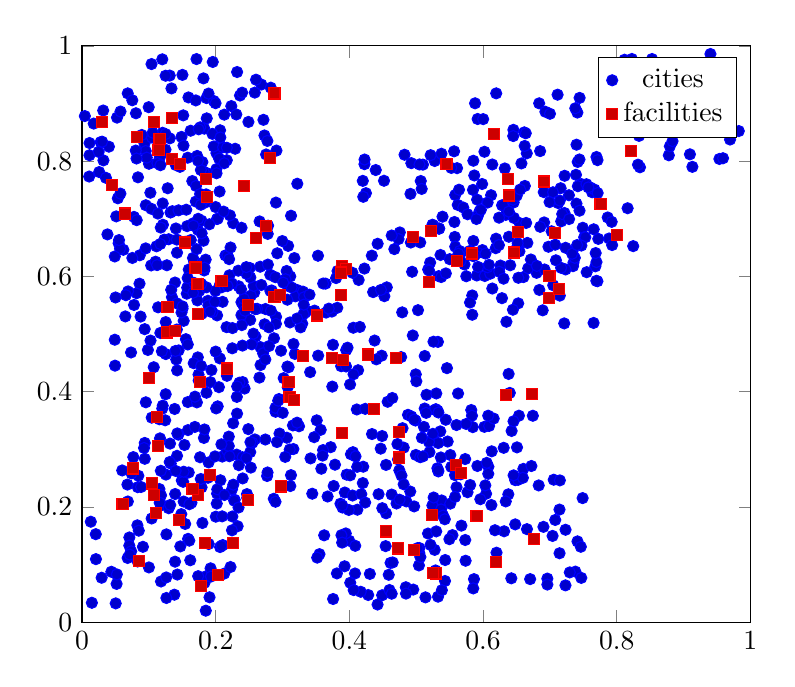
\begin{tikzpicture}
	\begin{axis}[
		width=0.7\textwidth,
		scale only axis,
		xmin=0,xmax=1,ymin=0,ymax=1,
		only marks]
		\addplot coordinates {
			(0.100138, 0.795319)
			(0.0278909, 0.832887)
			(0.386686, 0.205616)
			(0.228396, 0.212393)
			(0.70577, 0.247268)
			(0.149846, 0.254973)
			(0.246795, 0.222272)
			(0.224905, 0.1835)
			(0.642771, 0.331887)
			(0.760416, 0.754293)
			(0.186584, 0.874114)
			(0.741165, 0.884205)
			(0.433614, 0.635984)
			(0.226108, 0.345292)
			(0.562674, 0.396826)
			(0.0438895, 0.0875427)
			(0.311173, 0.520125)
			(0.333897, 0.537025)
			(0.638647, 0.668718)
			(0.134548, 0.563936)
			(0.172636, 0.558366)
			(0.74743, 0.759989)
			(0.103973, 0.968331)
			(0.539389, 0.703561)
			(0.512715, 0.370728)
			(0.158495, 0.333328)
			(0.188402, 0.557646)
			(0.182896, 0.856276)
			(0.142149, 0.288694)
			(0.358034, 0.266327)
			(0.202093, 0.532296)
			(0.3651, 0.53721)
			(0.186272, 0.909354)
			(0.645798, 0.72826)
			(0.206507, 0.130424)
			(0.763123, 0.746045)
			(0.227671, 0.210922)
			(0.201129, 0.813883)
			(0.712494, 0.727136)
			(0.660337, 0.266079)
			(0.205843, 0.747213)
			(0.556716, 0.816959)
			(0.723452, 0.160431)
			(0.199845, 0.720297)
			(0.581418, 0.641992)
			(0.183287, 0.0684819)
			(0.118171, 0.0707402)
			(0.146488, 0.790018)
			(0.405368, 0.295019)
			(0.693329, 0.885565)
			(0.69959, 0.728949)
			(0.54336, 0.107928)
			(0.908181, 0.893958)
			(0.0842425, 0.254142)
			(0.654476, 0.643529)
			(0.0934358, 0.830482)
			(0.164989, 0.765345)
			(0.0816917, 0.570847)
			(0.399748, 0.141499)
			(0.180056, 0.798329)
			(0.0939402, 0.283572)
			(0.173471, 0.680636)
			(0.735304, 0.62362)
			(0.46165, 0.102987)
			(0.351186, 0.350268)
			(0.148797, 0.841986)
			(0.210655, 0.13385)
			(0.19077, 0.043338)
			(0.484497, 0.060723)
			(0.530022, 0.202213)
			(0.891632, 0.873261)
			(0.149279, 0.24593)
			(0.243229, 0.405376)
			(0.0504015, 0.0327359)
			(0.142056, 0.553094)
			(0.651648, 0.65242)
			(0.186295, 0.0800304)
			(0.192334, 0.0935601)
			(0.464801, 0.103745)
			(0.132779, 0.275367)
			(0.602041, 0.338998)
			(0.741899, 0.756455)
			(0.274287, 0.317011)
			(0.53206, 0.36704)
			(0.896956, 0.911524)
			(0.150417, 0.544024)
			(0.265427, 0.424402)
			(0.170242, 0.576305)
			(0.0954244, 0.723432)
			(0.138157, 0.0477916)
			(0.0490077, 0.490102)
			(0.594817, 0.713226)
			(0.54426, 0.351267)
			(0.700138, 0.882069)
			(0.0402049, 0.825022)
			(0.598657, 0.760246)
			(0.144547, 0.471565)
			(0.734677, 0.617776)
			(0.271447, 0.871598)
			(0.116669, 0.318977)
			(0.206555, 0.586173)
			(0.152101, 0.522867)
			(0.278399, 0.68799)
			(0.442317, 0.656588)
			(0.0708031, 0.147078)
			(0.321841, 0.57641)
			(0.115763, 0.352163)
			(0.628508, 0.723306)
			(0.557746, 0.668437)
			(0.189028, 0.549716)
			(0.168837, 0.338813)
			(0.591149, 0.733149)
			(0.666352, 0.658085)
			(0.158298, 0.382002)
			(0.558373, 0.741121)
			(0.608008, 0.26982)
			(0.573272, 0.283101)
			(0.266868, 0.47732)
			(0.408771, 0.132641)
			(0.210368, 0.555825)
			(0.100055, 0.0951139)
			(0.178823, 0.622845)
			(0.308359, 0.652904)
			(0.599029, 0.645592)
			(0.474767, 0.263644)
			(0.749267, 0.684347)
			(0.714416, 0.19546)
			(0.648118, 0.246571)
			(0.188441, 0.250644)
			(0.174339, 0.429653)
			(0.517709, 0.153877)
			(0.277862, 0.673692)
			(0.274422, 0.543396)
			(0.154276, 0.659924)
			(0.115751, 0.231061)
			(0.644958, 0.733109)
			(0.111422, 0.652155)
			(0.402327, 0.291484)
			(0.283847, 0.575519)
			(0.613863, 0.57895)
			(0.216274, 0.511964)
			(0.00423215, 0.878114)
			(0.728536, 0.740806)
			(0.306426, 0.320108)
			(0.685431, 0.81732)
			(0.248783, 0.335009)
			(0.193594, 0.437498)
			(0.083249, 0.10548)
			(0.184974, 0.629)
			(0.289544, 0.365129)
			(0.893076, 0.913108)
			(0.319345, 0.565387)
			(0.307444, 0.583767)
			(0.592192, 0.640723)
			(0.457283, 0.382476)
			(0.424781, 0.744377)
			(0.591924, 0.873034)
			(0.65242, 0.247094)
			(0.216832, 0.427516)
			(0.224405, 0.230681)
			(0.185627, 0.742258)
			(0.454956, 0.188908)
			(0.0493631, 0.445141)
			(0.420112, 0.241461)
			(0.619526, 0.665375)
			(0.506833, 0.765443)
			(0.208606, 0.132522)
			(0.17564, 0.574959)
			(0.573363, 0.142699)
			(0.467324, 0.647336)
			(0.389709, 0.198959)
			(0.341922, 0.284253)
			(0.167762, 0.625598)
			(0.150221, 0.949571)
			(0.13381, 0.926092)
			(0.499505, 0.290242)
			(0.898034, 0.957643)
			(0.0618414, 0.646156)
			(0.176831, 0.858604)
			(0.458924, 0.0823489)
			(0.126231, 0.0421171)
			(0.318381, 0.465448)
			(0.357097, 0.333836)
			(0.411966, 0.195266)
			(0.42079, 0.738038)
			(0.499362, 0.430005)
			(0.0707725, 0.133035)
			(0.638278, 0.430763)
			(0.586456, 0.0748013)
			(0.661699, 0.849848)
			(0.766713, 0.75065)
			(0.690845, 0.746244)
			(0.547096, 0.313513)
			(0.226145, 0.69231)
			(0.428191, 0.0472675)
			(0.536039, 0.331071)
			(0.69787, 0.651383)
			(0.565108, 0.636426)
			(0.329507, 0.518043)
			(0.558053, 0.255189)
			(0.0864137, 0.636642)
			(0.289369, 0.371923)
			(0.0776882, 0.70322)
			(0.140947, 0.455796)
			(0.220543, 0.601916)
			(0.75135, 0.667859)
			(0.330605, 0.573526)
			(0.495606, 0.05668)
			(0.721494, 0.518428)
			(0.231963, 0.361886)
			(0.258639, 0.317145)
			(0.506004, 0.658857)
			(0.41114, 0.369112)
			(0.749009, 0.215363)
			(0.612502, 0.203321)
			(0.131236, 0.948384)
			(0.513858, 0.0431662)
			(0.250986, 0.614579)
			(0.422632, 0.794655)
			(0.257642, 0.57202)
			(0.116087, 0.819054)
			(0.093874, 0.311065)
			(0.259521, 0.495506)
			(0.214532, 0.636378)
			(0.690383, 0.165499)
			(0.19713, 0.825433)
			(0.200149, 0.183149)
			(0.173256, 0.459517)
			(0.171837, 0.381408)
			(0.515429, 0.394609)
			(0.449018, 0.323039)
			(0.504091, 0.0985542)
			(0.481352, 0.30299)
			(0.251558, 0.524428)
			(0.10474, 0.84081)
			(0.613771, 0.794131)
			(0.817939, 0.964138)
			(0.268293, 0.932849)
			(0.126939, 0.619321)
			(0.739765, 0.726224)
			(0.573942, 0.106711)
			(0.953663, 0.803707)
			(0.206189, 0.45775)
			(0.282385, 0.927387)
			(0.102259, 0.745079)
			(0.1513, 0.243628)
			(0.420094, 0.765678)
			(0.118177, 0.220241)
			(0.382324, 0.609309)
			(0.0547541, 0.657522)
			(0.487711, 0.359829)
			(0.433876, 0.326471)
			(0.0767337, 0.286456)
			(0.139336, 0.222441)
			(0.88989, 0.913564)
			(0.207001, 0.246312)
			(0.566616, 0.256619)
			(0.519835, 0.295134)
			(0.166291, 0.692047)
			(0.475495, 0.676273)
			(0.430672, 0.0838396)
			(0.200987, 0.786025)
			(0.103688, 0.717284)
			(0.532654, 0.0443652)
			(0.448344, 0.462402)
			(0.118865, 0.81432)
			(0.0688533, 0.573904)
			(0.353314, 0.462503)
			(0.714964, 0.246101)
			(0.374456, 0.408771)
			(0.401081, 0.412517)
			(0.188038, 0.778417)
			(0.206542, 0.853476)
			(0.765609, 0.681691)
			(0.529949, 0.157631)
			(0.744518, 0.909657)
			(0.316411, 0.482697)
			(0.209812, 0.28741)
			(0.753051, 0.667889)
			(0.153265, 0.307521)
			(0.801435, 0.888116)
			(0.307234, 0.55957)
			(0.572237, 0.62068)
			(0.294754, 0.387218)
			(0.0569541, 0.647924)
			(0.182145, 0.781488)
			(0.536377, 0.637135)
			(0.020808, 0.10949)
			(0.120069, 0.37064)
			(0.297732, 0.471074)
			(0.21766, 0.635966)
			(0.0985508, 0.47236)
			(0.372058, 0.303747)
			(0.691449, 0.693614)
			(0.347887, 0.540613)
			(0.131305, 0.839461)
			(0.0112746, 0.831349)
			(0.174534, 0.419309)
			(0.684256, 0.576471)
			(0.252518, 0.268263)
			(0.0647754, 0.530532)
			(0.159684, 0.611829)
			(0.270886, 0.466608)
			(0.126253, 0.15244)
			(0.0685147, 0.209477)
			(0.171303, 0.976994)
			(0.665429, 0.81349)
			(0.152097, 0.209335)
			(0.648146, 0.169778)
			(0.619016, 0.648921)
			(0.836954, 0.900841)
			(0.604584, 0.22288)
			(0.582395, 0.36816)
			(0.76979, 0.807115)
			(0.212696, 0.0843512)
			(0.722084, 0.774534)
			(0.261958, 0.543695)
			(0.479046, 0.537594)
			(0.620182, 0.120649)
			(0.564037, 0.750326)
			(0.654782, 0.692483)
			(0.267107, 0.446211)
			(0.741343, 0.140287)
			(0.723507, 0.612089)
			(0.538078, 0.211303)
			(0.914795, 0.968621)
			(0.637848, 0.221955)
			(0.811683, 0.975793)
			(0.492709, 0.796446)
			(0.57494, 0.600215)
			(0.583848, 0.566949)
			(0.151811, 0.826926)
			(0.634023, 0.706673)
			(0.629842, 0.723086)
			(0.413896, 0.593779)
			(0.0131008, 0.174382)
			(0.73374, 0.6428)
			(0.158187, 0.805898)
			(0.393215, 0.225061)
			(0.355234, 0.118135)
			(0.585372, 0.0587001)
			(0.824694, 0.65248)
			(0.584666, 0.338504)
			(0.551054, 0.290102)
			(0.144146, 0.325446)
			(0.982692, 0.852115)
			(0.113847, 0.546322)
			(0.253968, 0.482136)
			(0.170258, 0.729833)
			(0.683973, 0.900224)
			(0.197147, 0.904266)
			(0.202996, 0.374533)
			(0.201598, 0.205844)
			(0.59071, 0.601547)
			(0.602595, 0.600688)
			(0.524194, 0.20264)
			(0.500204, 0.418043)
			(0.534266, 0.682672)
			(0.252706, 0.566793)
			(0.301685, 0.423468)
			(0.170531, 0.756874)
			(0.716144, 0.752967)
			(0.493889, 0.607992)
			(0.471939, 0.309137)
			(0.290356, 0.529717)
			(0.322109, 0.760725)
			(0.178854, 0.234175)
			(0.905, 0.87355)
			(0.504603, 0.120088)
			(0.525585, 0.68859)
			(0.336133, 0.540228)
			(0.38137, 0.0847279)
			(0.364367, 0.587445)
			(0.177836, 0.784569)
			(0.689267, 0.541093)
			(0.409179, 0.287773)
			(0.231334, 0.290795)
			(0.623764, 0.6543)
			(0.413074, 0.437211)
			(0.282627, 0.540316)
			(0.125169, 0.39555)
			(0.217475, 0.636337)
			(0.672369, 0.271045)
			(0.178757, 0.696534)
			(0.70468, 0.745905)
			(0.159627, 0.259806)
			(0.612043, 0.740801)
			(0.844462, 0.960745)
			(0.167118, 0.449409)
			(0.240353, 0.249494)
			(0.202091, 0.223235)
			(0.472794, 0.282474)
			(0.119433, 0.203252)
			(0.721892, 0.709931)
			(0.422778, 0.802683)
			(0.626067, 0.618755)
			(0.251685, 0.295214)
			(0.141847, 0.507808)
			(0.132413, 0.710799)
			(0.533681, 0.600461)
			(0.22912, 0.821405)
			(0.256799, 0.583528)
			(0.147052, 0.131579)
			(0.437797, 0.488685)
			(0.741625, 0.798519)
			(0.176661, 0.74295)
			(0.449022, 0.0468219)
			(0.0490135, 0.634537)
			(0.744278, 0.802838)
			(0.670502, 0.074832)
			(0.529465, 0.369562)
			(0.401333, 0.0685008)
			(0.772479, 0.665055)
			(0.151398, 0.879329)
			(0.492767, 0.357036)
			(0.708016, 0.177464)
			(0.182365, 0.319742)
			(0.309109, 0.442445)
			(0.157212, 0.687146)
			(0.201941, 0.69954)
			(0.216575, 0.801514)
			(0.135101, 0.713067)
			(0.56763, 0.167567)
			(0.313689, 0.580747)
			(0.189366, 0.277317)
			(0.380138, 0.597066)
			(0.395948, 0.256044)
			(0.260346, 0.941202)
			(0.662319, 0.826276)
			(0.176523, 0.286269)
			(0.226401, 0.238688)
			(0.142555, 0.327576)
			(0.240154, 0.286257)
			(0.0320141, 0.801264)
			(0.663929, 0.848265)
			(0.0523494, 0.875428)
			(0.716847, 0.614805)
			(0.834821, 0.789257)
			(0.52087, 0.623905)
			(0.527637, 0.125544)
			(0.53741, 0.59889)
			(0.0293439, 0.0772011)
			(0.404556, 0.606265)
			(0.307233, 0.443545)
			(0.238487, 0.532914)
			(0.238528, 0.555291)
			(0.609098, 0.340622)
			(0.286913, 0.214186)
			(0.251857, 0.598162)
			(0.246123, 0.60443)
			(0.640643, 0.619255)
			(0.154346, 0.170554)
			(0.579545, 0.643718)
			(0.714871, 0.566618)
			(0.125348, 0.465215)
			(0.199762, 0.900452)
			(0.527919, 0.368443)
			(0.331378, 0.534786)
			(0.208891, 0.581125)
			(0.452355, 0.565673)
			(0.152104, 0.26116)
			(0.58549, 0.661422)
			(0.102452, 0.488636)
			(0.113478, 0.70893)
			(0.373802, 0.538926)
			(0.498959, 0.349972)
			(0.652637, 0.553222)
			(0.680136, 0.606166)
			(0.129698, 0.664429)
			(0.0954264, 0.381568)
			(0.531701, 0.267096)
			(0.696228, 0.0757104)
			(0.292128, 0.640079)
			(0.491082, 0.226799)
			(0.771126, 0.591601)
			(0.120578, 0.84913)
			(0.195124, 0.847233)
			(0.600184, 0.8728)
			(0.324672, 0.339975)
			(0.166021, 0.63193)
			(0.392878, 0.0970875)
			(0.055323, 0.662999)
			(0.737296, 0.632196)
			(0.504748, 0.12873)
			(0.512772, 0.461881)
			(0.650822, 0.303374)
			(0.0111302, 0.810159)
			(0.315587, 0.341449)
			(0.612996, 0.296537)
			(0.0735594, 0.123031)
			(0.272947, 0.84448)
			(0.178097, 0.444683)
			(0.210922, 0.824075)
			(0.148876, 0.537484)
			(0.307801, 0.407715)
			(0.181808, 0.661865)
			(0.162749, 0.66306)
			(0.714827, 0.731463)
			(0.451832, 0.76586)
			(0.660543, 0.598826)
			(0.20305, 0.700222)
			(0.221302, 0.705818)
			(0.199967, 0.469476)
			(0.562214, 0.723992)
			(0.081758, 0.697562)
			(0.0300935, 0.833637)
			(0.591571, 0.271105)
			(0.204811, 0.407846)
			(0.723358, 0.0639898)
			(0.634013, 0.209633)
			(0.290129, 0.51769)
			(0.156746, 0.569986)
			(0.0952517, 0.817484)
			(0.234388, 0.582886)
			(0.277339, 0.835016)
			(0.138605, 0.370005)
			(0.517948, 0.611994)
			(0.533122, 0.261668)
			(0.125514, 0.256122)
			(0.327014, 0.511567)
			(0.116219, 0.207351)
			(0.768095, 0.61746)
			(0.11718, 0.501887)
			(0.527722, 0.800191)
			(0.189271, 0.917118)
			(0.290871, 0.818241)
			(0.417037, 0.0528264)
			(0.0248352, 0.815955)
			(0.645429, 0.85423)
			(0.610748, 0.604601)
			(0.558426, 0.651597)
			(0.514953, 0.363197)
			(0.159262, 0.910464)
			(0.0937663, 0.508477)
			(0.969635, 0.83741)
			(0.182806, 0.610283)
			(0.321792, 0.346217)
			(0.074133, 0.258235)
			(0.289448, 0.209019)
			(0.290147, 0.728032)
			(0.566386, 0.626737)
			(0.653719, 0.358324)
			(0.232035, 0.954515)
			(0.254981, 0.311357)
			(0.158634, 0.144659)
			(0.378489, 0.27331)
			(0.580543, 0.554639)
			(0.245793, 0.284902)
			(0.537284, 0.195674)
			(0.141831, 0.663799)
			(0.521439, 0.134158)
			(0.606748, 0.61582)
			(0.640054, 0.397863)
			(0.662573, 0.756922)
			(0.422518, 0.613543)
			(0.104289, 0.354954)
			(0.025643, 0.781008)
			(0.696262, 0.0653663)
			(0.162512, 0.852674)
			(0.126006, 0.0777105)
			(0.360631, 0.29869)
			(0.116514, 0.806617)
			(0.185172, 0.0200894)
			(0.359985, 0.289092)
			(0.554257, 0.151182)
			(0.739073, 0.776184)
			(0.144371, 0.714587)
			(0.0379972, 0.672838)
			(0.456011, 0.580994)
			(0.212819, 0.880549)
			(0.0683833, 0.917486)
			(0.0837142, 0.771844)
			(0.273182, 0.516886)
			(0.667591, 0.613984)
			(0.295516, 0.327322)
			(0.316249, 0.300454)
			(0.225115, 0.510293)
			(0.198552, 0.555901)
			(0.341293, 0.433883)
			(0.532523, 0.486397)
			(0.550125, 0.629854)
			(0.443717, 0.222135)
			(0.181691, 0.943504)
			(0.14262, 0.0827359)
			(0.73818, 0.0878293)
			(0.125259, 0.520702)
			(0.649742, 0.64564)
			(0.585526, 0.800596)
			(0.360796, 0.587606)
			(0.142319, 0.436949)
			(0.195072, 0.538067)
			(0.131646, 0.309887)
			(0.510086, 0.793877)
			(0.536883, 0.285891)
			(0.405898, 0.510896)
			(0.256378, 0.500617)
			(0.376539, 0.236407)
			(0.381927, 0.545519)
			(0.201215, 0.778925)
			(0.184596, 0.728282)
			(0.0517235, 0.0665383)
			(0.240322, 0.416623)
			(0.311557, 0.599981)
			(0.0804015, 0.818288)
			(0.624166, 0.608043)
			(0.913247, 0.790029)
			(0.550925, 0.205761)
			(0.236342, 0.913769)
			(0.129651, 0.197837)
			(0.0968508, 0.806054)
			(0.265691, 0.695383)
			(0.0752192, 0.905532)
			(0.816354, 0.718211)
			(0.161953, 0.107547)
			(0.528932, 0.0898808)
			(0.180088, 0.172177)
			(0.464266, 0.38902)
			(0.20235, 0.230644)
			(0.192893, 0.0792552)
			(0.557185, 0.694337)
			(0.511545, 0.338889)
			(0.209586, 0.183685)
			(0.0911247, 0.130845)
			(0.199623, 0.574802)
			(0.755106, 0.607271)
			(0.744392, 0.713953)
			(0.293483, 0.384371)
			(0.274264, 0.455851)
			(0.904353, 0.936024)
			(0.125062, 0.948071)
			(0.235561, 0.415629)
			(0.190509, 0.690402)
			(0.0501327, 0.563427)
			(0.406257, 0.430252)
			(0.583451, 0.358293)
			(0.63092, 0.302586)
			(0.0753005, 0.631983)
			(0.179146, 0.535086)
			(0.281658, 0.60281)
			(0.241664, 0.548887)
			(0.771466, 0.744605)
			(0.231648, 0.390933)
			(0.532927, 0.310904)
			(0.089416, 0.845342)
			(0.75476, 0.759909)
			(0.449283, 0.197872)
			(0.420743, 0.26984)
			(0.0997394, 0.893537)
			(0.0806495, 0.882939)
			(0.387727, 0.444224)
			(0.460021, 0.055915)
			(0.532866, 0.263527)
			(0.608904, 0.61994)
			(0.124962, 0.846863)
			(0.0316399, 0.887769)
			(0.850688, 0.968362)
			(0.173823, 0.699864)
			(0.239542, 0.918723)
			(0.310803, 0.299721)
			(0.519202, 0.610164)
			(0.878004, 0.810094)
			(0.168957, 0.391359)
			(0.157331, 0.58053)
			(0.219614, 0.322025)
			(0.139102, 0.589333)
			(0.606874, 0.728108)
			(0.470602, 0.206004)
			(0.40481, 0.219865)
			(0.519063, 0.312915)
			(0.103433, 0.619032)
			(0.18317, 0.334454)
			(0.757576, 0.754455)
			(0.704045, 0.149765)
			(0.491438, 0.743135)
			(0.819665, 0.880531)
			(0.723549, 0.649598)
			(0.940258, 0.985773)
			(0.394638, 0.154082)
			(0.583852, 0.533436)
			(0.494922, 0.497482)
			(0.150232, 0.547941)
			(0.142126, 0.641121)
			(0.408434, 0.0845818)
			(0.110011, 0.625467)
			(0.72981, 0.0864926)
			(0.242268, 0.56111)
			(0.155396, 0.491095)
			(0.576823, 0.225605)
			(0.733355, 0.63926)
			(0.116279, 0.794876)
			(0.22336, 0.89542)
			(0.388185, 0.15107)
			(0.508522, 0.319999)
			(0.506253, 0.113179)
			(0.852883, 0.977085)
			(0.521602, 0.81027)
			(0.401135, 0.254881)
			(0.496954, 0.351555)
			(0.508218, 0.751752)
			(0.312645, 0.255191)
			(0.0679079, 0.238839)
			(0.121067, 0.689528)
			(0.191671, 0.53915)
			(0.128125, 0.752885)
			(0.747145, 0.653484)
			(0.44036, 0.456061)
			(0.879568, 0.825751)
			(0.584976, 0.750054)
			(0.0655766, 0.567376)
			(0.0682508, 0.111544)
			(0.198978, 0.287716)
			(0.651868, 0.657532)
			(0.570432, 0.719481)
			(0.237976, 0.577681)
			(0.959096, 0.804961)
			(0.395051, 0.443716)
			(0.524962, 0.326842)
			(0.24005, 0.479908)
			(0.123035, 0.663736)
			(0.25847, 0.918813)
			(0.39524, 0.472199)
			(0.367467, 0.218126)
			(0.120079, 0.976559)
			(0.300252, 0.363227)
			(0.183218, 0.614999)
			(0.166194, 0.571498)
			(0.533268, 0.363808)
			(0.399216, 0.194827)
			(0.312754, 0.705222)
			(0.0575291, 0.885972)
			(0.607824, 0.257531)
			(0.786545, 0.70222)
			(0.0815375, 0.804512)
			(0.220042, 0.629915)
			(0.131927, 0.203466)
			(0.35306, 0.635833)
			(0.646222, 0.701418)
			(0.502224, 0.128683)
			(0.195589, 0.971993)
			(0.615914, 0.353355)
			(0.306147, 0.609385)
			(0.634947, 0.521277)
			(0.11232, 0.61957)
			(0.171388, 0.647126)
			(0.239087, 0.515455)
			(0.645635, 0.348679)
			(0.644731, 0.542183)
			(0.664506, 0.692727)
			(0.525879, 0.486668)
			(0.224809, 0.475227)
			(0.705013, 0.584544)
			(0.177704, 0.248451)
			(0.595966, 0.213444)
			(0.0860255, 0.587359)
			(0.112719, 0.796407)
			(0.955769, 0.883423)
			(0.206935, 0.841027)
			(0.534385, 0.683155)
			(0.642326, 0.0762271)
			(0.709083, 0.627897)
			(0.0828281, 0.168137)
			(0.739891, 0.828436)
			(0.16764, 0.588709)
			(0.117243, 0.792866)
			(0.463367, 0.221501)
			(0.623976, 0.701853)
			(0.505989, 0.286335)
			(0.216634, 0.298807)
			(0.10729, 0.442375)
			(0.716949, 0.695482)
			(0.287201, 0.492626)
			(0.0952369, 0.648564)
			(0.587714, 0.636822)
			(0.299705, 0.661261)
			(0.177783, 0.724281)
			(0.605548, 0.276486)
			(0.397239, 0.476331)
			(0.173773, 0.079951)
			(0.344501, 0.222979)
			(0.276926, 0.253715)
			(0.544362, 0.605129)
			(0.251973, 0.3124)
			(0.504919, 0.794161)
			(0.375448, 0.481333)
			(0.560299, 0.342118)
			(0.909577, 0.811727)
			(0.588101, 0.900277)
			(0.259248, 0.543221)
			(0.473535, 0.664728)
			(0.746312, 0.130917)
			(0.526112, 0.21641)
			(0.485185, 0.209701)
			(0.140247, 0.793285)
			(0.477476, 0.459995)
			(0.482571, 0.811022)
			(0.463331, 0.0495021)
			(0.117098, 0.656154)
			(0.417861, 0.222231)
			(0.463374, 0.670892)
			(0.369212, 0.544037)
			(0.332093, 0.563814)
			(0.281809, 0.574761)
			(0.192051, 0.416526)
			(0.74082, 0.654372)
			(0.13125, 0.278)
			(0.576823, 0.707806)
			(0.351885, 0.112099)
			(0.232791, 0.16656)
			(0.0106942, 0.773207)
			(0.692065, 0.612009)
			(0.524326, 0.689623)
			(0.200648, 0.370964)
			(0.632606, 0.787229)
			(0.311635, 0.236298)
			(0.702619, 0.678243)
			(0.104171, 0.180004)
			(0.0713314, 0.117371)
			(0.475104, 0.212587)
			(0.650406, 0.740025)
			(0.185194, 0.734851)
			(0.442196, 0.0307709)
			(0.714501, 0.119706)
			(0.652857, 0.597542)
			(0.769557, 0.592283)
			(0.63074, 0.596038)
			(0.592289, 0.705164)
			(0.718497, 0.708089)
			(0.552482, 0.269514)
			(0.746999, 0.0769671)
			(0.304035, 0.286881)
			(0.124844, 0.81977)
			(0.801565, 0.932952)
			(0.16372, 0.207341)
			(0.247191, 0.215746)
			(0.211849, 0.712366)
			(0.665727, 0.161519)
			(0.565162, 0.644021)
			(0.411731, 0.269616)
			(0.213065, 0.220809)
			(0.769722, 0.624812)
			(0.230795, 0.880902)
			(0.543082, 0.0715518)
			(0.560393, 0.23419)
			(0.585397, 0.635112)
			(0.266574, 0.616798)
			(0.140034, 0.262543)
			(0.139773, 0.470585)
			(0.18621, 0.580988)
			(0.537794, 0.812739)
			(0.78855, 0.665692)
			(0.831876, 0.793748)
			(0.628341, 0.562207)
			(0.435555, 0.572721)
			(0.883492, 0.834636)
			(0.638618, 0.712378)
			(0.340309, 0.568283)
			(0.833411, 0.843726)
			(0.477949, 0.254537)
			(0.0927555, 0.302345)
			(0.825016, 0.884308)
			(0.24378, 0.540272)
			(0.0849266, 0.158866)
			(0.683334, 0.23735)
			(0.389184, 0.138177)
			(0.481239, 0.239306)
			(0.0834232, 0.234366)
			(0.574719, 0.343983)
			(0.540272, 0.18511)
			(0.279589, 0.511569)
			(0.561133, 0.787754)
			(0.659609, 0.2505)
			(0.222164, 0.0958092)
			(0.0535344, 0.735484)
			(0.105738, 0.84929)
			(0.54281, 0.178684)
			(0.563239, 0.639236)
			(0.0520683, 0.08307)
			(0.120709, 0.726528)
			(0.454265, 0.13205)
			(0.304478, 0.595072)
			(0.0733456, 0.468019)
			(0.602127, 0.816156)
			(0.119494, 0.470005)
			(0.491972, 0.658743)
			(0.415638, 0.512325)
			(0.189562, 0.135774)
			(0.268292, 0.5851)
			(0.289176, 0.598626)
			(0.219596, 0.305767)
			(0.205071, 0.804367)
			(0.937965, 0.944399)
			(0.55811, 0.217357)
			(0.631556, 0.157813)
			(0.496915, 0.200974)
			(0.530047, 0.396889)
			(0.552536, 0.788162)
			(0.711569, 0.915184)
			(0.0205545, 0.152775)
			(0.158237, 0.48187)
			(0.619697, 0.917509)
			(0.0573995, 0.743592)
			(0.645735, 0.254828)
			(0.439468, 0.7845)
			(0.655588, 0.750633)
			(0.148514, 0.187602)
			(0.22225, 0.65012)
			(0.423722, 0.370172)
			(0.170207, 0.90527)
			(0.0357307, 0.770979)
			(0.538431, 0.0556244)
			(0.186187, 0.398134)
			(0.423614, 0.207674)
			(0.728778, 0.699479)
			(0.224388, 0.159469)
			(0.484734, 0.0496875)
			(0.822716, 0.977173)
			(0.80456, 0.887117)
			(0.592589, 0.616409)
			(0.0778097, 0.550426)
			(0.234147, 0.198961)
			(0.051167, 0.704087)
			(0.590098, 0.699536)
			(0.607758, 0.358322)
			(0.32179, 0.526922)
			(0.224193, 0.587743)
			(0.771252, 0.801652)
			(0.279737, 0.479161)
			(0.54968, 0.144112)
			(0.166711, 0.688075)
			(0.474431, 0.283037)
			(0.0876298, 0.530244)
			(0.580746, 0.238078)
			(0.301064, 0.589195)
			(0.0882765, 0.234644)
			(0.139196, 0.105096)
			(0.120733, 0.375743)
			(0.16046, 0.141585)
			(0.220527, 0.288036)
			(0.707989, 0.654904)
			(0.502717, 0.541393)
			(0.674522, 0.358224)
			(0.793176, 0.654324)
			(0.586914, 0.775084)
			(0.216693, 0.823105)
			(0.160562, 0.204821)
			(0.217682, 0.583255)
			(0.671571, 0.629294)
			(0.362297, 0.150794)
			(0.685587, 0.685971)
			(0.765415, 0.519233)
			(0.174507, 0.855171)
			(0.248963, 0.867958)
			(0.375669, 0.0403373)
			(0.792473, 0.694594)
			(0.277597, 0.259815)
			(0.234583, 0.272503)
			(0.454865, 0.272955)
			(0.155935, 0.715651)
			(0.233738, 0.609864)
			(0.44728, 0.576558)
			(0.178487, 0.58695)
			(0.172224, 0.808974)
			(0.768521, 0.640446)
			(0.479569, 0.336653)
			(0.657437, 0.795976)
			(0.238648, 0.684345)
			(0.645183, 0.843433)
			(0.117802, 0.684607)
			(0.406445, 0.0558214)
			(0.291709, 0.312601)
			(0.275401, 0.811505)
			(0.124432, 0.350343)
			(0.446912, 0.301165)
			(0.158016, 0.597075)
			(0.0600986, 0.263346)
			(0.738047, 0.891627)
			(0.232131, 0.40903)
			(0.133425, 0.576682)
			(0.596759, 0.715462)
			(0.20854, 0.308642)
			(0.603634, 0.639519)
			(0.331733, 0.550942)
			(0.24576, 0.616061)
			(0.617853, 0.159628)
			(0.317704, 0.631738)
			(0.849558, 0.891246)
			(0.0174753, 0.8651)
			(0.178973, 0.674766)
			(0.173621, 0.800632)
			(0.389451, 0.202439)
			(0.0147158, 0.0337685)
			(0.546022, 0.440791)
			(0.117914, 0.262674)
			(0.347342, 0.321107)
			(0.603391, 0.237481)
			(0.140423, 0.683102)
			(0.680443, 0.618229)
			(0.278082, 0.620409)
			(0.21278, 0.796296)
			(0.510125, 0.287849)
		};
		\addlegendentry{cities}
		\addplot coordinates {
			(0.388868, 0.327816)
			(0.496999, 0.125771)
			(0.192036, 0.255178)
			(0.135216, 0.874212)
			(0.288001, 0.917323)
			(0.634861, 0.393873)
			(0.69071, 0.764609)
			(0.676196, 0.144022)
			(0.387317, 0.567882)
			(0.871209, 0.897182)
			(0.110633, 0.189431)
			(0.454719, 0.157555)
			(0.559598, 0.272752)
			(0.172738, 0.586294)
			(0.351206, 0.532171)
			(0.469859, 0.458932)
			(0.105025, 0.240848)
			(0.390358, 0.455156)
			(0.472337, 0.127976)
			(0.187504, 0.738287)
			(0.28794, 0.563736)
			(0.566481, 0.259381)
			(0.437312, 0.370115)
			(0.545341, 0.79555)
			(0.0768625, 0.266841)
			(0.518973, 0.590264)
			(0.495597, 0.668815)
			(0.523216, 0.186258)
			(0.698848, 0.562439)
			(0.388396, 0.617826)
			(0.619448, 0.104351)
			(0.473779, 0.329565)
			(0.208781, 0.591742)
			(0.226169, 0.137694)
			(0.474513, 0.285744)
			(0.373558, 0.458069)
			(0.108215, 0.220275)
			(0.699378, 0.60059)
			(0.173964, 0.220911)
			(0.21717, 0.440051)
			(0.281739, 0.805702)
			(0.173125, 0.534372)
			(0.0296354, 0.86782)
			(0.165412, 0.230741)
			(0.127595, 0.502757)
			(0.0640538, 0.709042)
			(0.16987, 0.615292)
			(0.111866, 0.355824)
			(0.183968, 0.137422)
			(0.583275, 0.639696)
			(0.561004, 0.626914)
			(0.42746, 0.464409)
			(0.310471, 0.390971)
			(0.0444417, 0.758864)
			(0.114205, 0.306348)
			(0.638965, 0.740348)
			(0.530052, 0.0847015)
			(0.0606401, 0.205678)
			(0.672975, 0.396386)
			(0.330162, 0.461867)
			(0.297858, 0.235541)
			(0.522264, 0.678752)
			(0.821687, 0.817248)
			(0.274702, 0.687603)
			(0.939718, 0.950835)
			(0.247929, 0.550724)
			(0.0853396, 0.106837)
			(0.652494, 0.676362)
			(0.241775, 0.757197)
			(0.100061, 0.423312)
			(0.14475, 0.176875)
			(0.8008, 0.671588)
			(0.114473, 0.818604)
			(0.139709, 0.505509)
			(0.395176, 0.612104)
			(0.203236, 0.081571)
			(0.248412, 0.212638)
			(0.524769, 0.0861466)
			(0.128009, 0.546726)
			(0.590278, 0.184234)
			(0.18591, 0.769436)
			(0.134503, 0.804303)
			(0.637663, 0.768339)
			(0.646767, 0.64145)
			(0.775793, 0.725558)
			(0.616526, 0.846619)
			(0.387504, 0.606673)
			(0.17603, 0.417349)
			(0.260767, 0.666162)
			(0.707648, 0.675211)
			(0.317696, 0.385031)
			(0.178288, 0.0634958)
			(0.296377, 0.567289)
			(0.107673, 0.868137)
			(0.146028, 0.795104)
			(0.71379, 0.578606)
			(0.0821275, 0.841814)
			(0.115973, 0.838736)
			(0.153502, 0.658803)
			(0.309042, 0.416121)
		};
		\addlegendentry{facilities}
	\end{axis}
	\end{tikzpicture}
\end{figure}
\pgfsetplotmarksize{2pt}
\begin{figure}
	\centering
 \caption{\label{FLClustered/test4.txt}FLClustered/test4.txt},
	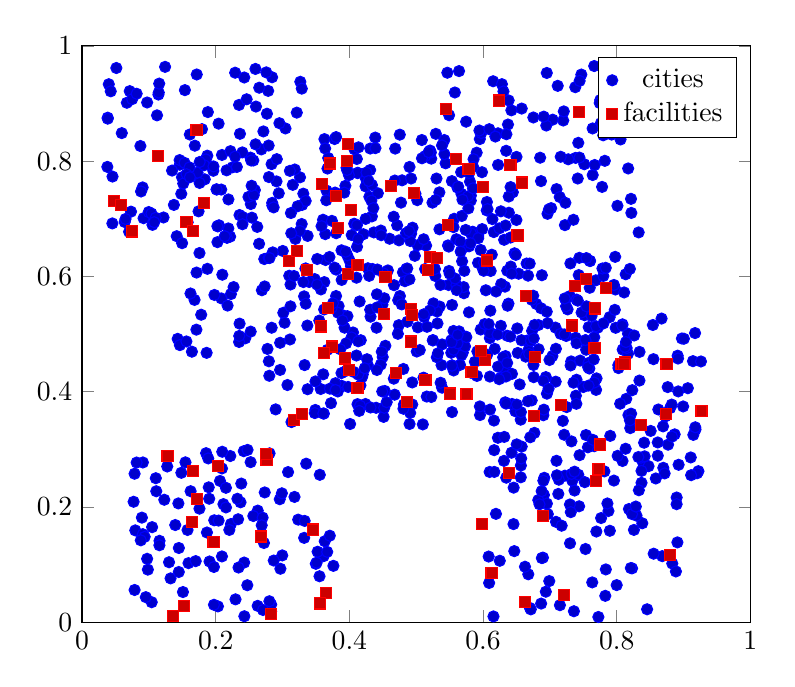
\begin{tikzpicture}
	\begin{axis}[
		width=0.7\textwidth,
		scale only axis,
		xmin=0,xmax=1,ymin=0,ymax=1,
		only marks]
		\addplot coordinates {
			(0.744096, 0.632171)
			(0.208481, 0.561811)
			(0.242006, 0.296775)
			(0.751917, 0.532667)
			(0.475592, 0.565975)
			(0.656471, 0.251456)
			(0.768767, 0.59316)
			(0.845522, 0.0225129)
			(0.159309, 0.102578)
			(0.605554, 0.714439)
			(0.564108, 0.956155)
			(0.0638331, 0.694383)
			(0.818303, 0.196401)
			(0.816919, 0.500639)
			(0.417045, 0.489263)
			(0.388485, 0.59386)
			(0.683181, 0.473616)
			(0.310031, 0.601075)
			(0.87996, 0.37153)
			(0.529392, 0.847227)
			(0.634739, 0.250777)
			(0.0771711, 0.209006)
			(0.271348, 0.851481)
			(0.236299, 0.847317)
			(0.328678, 0.690824)
			(0.514846, 0.653437)
			(0.787665, 0.193)
			(0.326152, 0.771856)
			(0.564172, 0.504592)
			(0.269097, 0.575961)
			(0.889724, 0.216398)
			(0.273366, 0.225213)
			(0.596528, 0.507842)
			(0.555693, 0.595495)
			(0.515817, 0.391518)
			(0.769853, 0.423075)
			(0.427785, 0.614073)
			(0.581829, 0.740197)
			(0.75003, 0.408082)
			(0.690272, 0.3591)
			(0.284381, 0.945445)
			(0.268328, 0.820301)
			(0.530342, 0.769725)
			(0.65664, 0.271884)
			(0.87312, 0.357227)
			(0.675871, 0.425195)
			(0.696481, 0.708522)
			(0.720013, 0.870388)
			(0.635169, 0.434841)
			(0.657096, 0.284156)
			(0.798075, 0.577256)
			(0.747101, 0.950129)
			(0.412584, 0.779748)
			(0.110384, 0.249885)
			(0.553403, 0.765255)
			(0.179496, 0.855377)
			(0.395844, 0.788382)
			(0.644619, 0.745868)
			(0.412197, 0.378356)
			(0.244217, 0.492511)
			(0.808951, 0.472942)
			(0.691168, 0.220773)
			(0.787646, 0.94158)
			(0.731935, 0.452475)
			(0.616117, 0.676865)
			(0.376104, 0.0978532)
			(0.838298, 0.171721)
			(0.569731, 0.467805)
			(0.689604, 0.112127)
			(0.22964, 0.0397281)
			(0.348146, 0.595303)
			(0.834159, 0.469003)
			(0.899447, 0.374364)
			(0.638024, 0.552747)
			(0.429943, 0.738084)
			(0.457589, 0.610366)
			(0.754071, 0.324777)
			(0.449431, 0.550659)
			(0.308279, 0.260519)
			(0.567681, 0.743248)
			(0.295888, 0.21343)
			(0.0910574, 0.277188)
			(0.0732562, 0.712312)
			(0.489998, 0.789835)
			(0.548345, 0.585085)
			(0.318329, 0.785403)
			(0.632836, 0.582196)
			(0.0786669, 0.0559714)
			(0.144161, 0.206157)
			(0.571428, 0.570801)
			(0.203276, 0.686898)
			(0.6827, 0.211953)
			(0.388194, 0.432262)
			(0.329381, 0.723986)
			(0.733606, 0.245507)
			(0.590461, 0.814599)
			(0.259473, 0.959874)
			(0.615133, 0.938508)
			(0.869733, 0.267916)
			(0.542079, 0.836526)
			(0.394017, 0.757059)
			(0.424045, 0.378595)
			(0.622512, 0.443422)
			(0.792434, 0.846065)
			(0.247636, 0.298979)
			(0.363164, 0.140506)
			(0.388259, 0.410277)
			(0.82962, 0.184926)
			(0.546604, 0.953305)
			(0.745348, 0.453916)
			(0.63132, 0.279965)
			(0.148599, 0.259261)
			(0.304375, 0.856664)
			(0.13249, 0.0761024)
			(0.570995, 0.581472)
			(0.609694, 0.503691)
			(0.153921, 0.9231)
			(0.440055, 0.372033)
			(0.675449, 0.446335)
			(0.682798, 0.515567)
			(0.121937, 0.702196)
			(0.642409, 0.888093)
			(0.651974, 0.467225)
			(0.362259, 0.542638)
			(0.769167, 0.403103)
			(0.808732, 0.279768)
			(0.0973973, 0.110027)
			(0.667873, 0.471919)
			(0.442619, 0.744137)
			(0.500852, 0.469633)
			(0.867155, 0.526811)
			(0.537967, 0.446035)
			(0.494079, 0.377773)
			(0.574307, 0.495471)
			(0.203331, 0.0275237)
			(0.780033, 0.600768)
			(0.790102, 0.920189)
			(0.420118, 0.430008)
			(0.46021, 0.665303)
			(0.478819, 0.76663)
			(0.209415, 0.266835)
			(0.665206, 0.488288)
			(0.411453, 0.651275)
			(0.380148, 0.611719)
			(0.449869, 0.460068)
			(0.436609, 0.676287)
			(0.657539, 0.48928)
			(0.451249, 0.356275)
			(0.123074, 0.212506)
			(0.654795, 0.412543)
			(0.296808, 0.0927957)
			(0.09066, 0.754343)
			(0.337557, 0.670223)
			(0.14849, 0.743284)
			(0.922277, 0.262057)
			(0.319189, 0.665055)
			(0.405504, 0.502732)
			(0.552465, 0.489096)
			(0.252076, 0.806023)
			(0.636285, 0.497018)
			(0.157876, 0.160102)
			(0.530867, 0.459767)
			(0.143075, 0.491604)
			(0.391191, 0.531966)
			(0.242696, 0.945032)
			(0.647153, 0.640073)
			(0.130185, 0.104111)
			(0.362514, 0.590048)
			(0.671601, 0.48824)
			(0.141698, 0.669702)
			(0.485255, 0.613095)
			(0.30116, 0.53685)
			(0.861485, 0.288934)
			(0.403284, 0.494146)
			(0.466499, 0.422532)
			(0.416035, 0.375657)
			(0.168346, 0.778425)
			(0.235641, 0.706417)
			(0.282926, 0.0188693)
			(0.703784, 0.461849)
			(0.634594, 0.817885)
			(0.679753, 0.552099)
			(0.300343, 0.644119)
			(0.209356, 0.11418)
			(0.355355, 0.0797836)
			(0.158055, 0.693902)
			(0.452323, 0.562027)
			(0.262815, 0.0284254)
			(0.543999, 0.796137)
			(0.595461, 0.359441)
			(0.663971, 0.460747)
			(0.665219, 0.622244)
			(0.362721, 0.838105)
			(0.591477, 0.469862)
			(0.56725, 0.780781)
			(0.766291, 0.305435)
			(0.775387, 0.905893)
			(0.471492, 0.688631)
			(0.709133, 0.174175)
			(0.669805, 0.622221)
			(0.433707, 0.704016)
			(0.295349, 0.865731)
			(0.11109, 0.22726)
			(0.434696, 0.612777)
			(0.429615, 0.600903)
			(0.742533, 0.83165)
			(0.580517, 0.764231)
			(0.0378928, 0.789943)
			(0.2785, 0.921799)
			(0.610223, 0.492984)
			(0.754225, 0.47273)
			(0.0796673, 0.15937)
			(0.492337, 0.769783)
			(0.432881, 0.731447)
			(0.693979, 0.42529)
			(0.414733, 0.366646)
			(0.61638, 0.349855)
			(0.209372, 0.810641)
			(0.742573, 0.255928)
			(0.85081, 0.331914)
			(0.614824, 0.499914)
			(0.582106, 0.432759)
			(0.183684, 0.768351)
			(0.892078, 0.400471)
			(0.357428, 0.577385)
			(0.920385, 0.258475)
			(0.596513, 0.645868)
			(0.285336, 0.641639)
			(0.189578, 0.234058)
			(0.738471, 0.805531)
			(0.407592, 0.820486)
			(0.595229, 0.838239)
			(0.722545, 0.688913)
			(0.172888, 0.779818)
			(0.613076, 0.637639)
			(0.222806, 0.569269)
			(0.649105, 0.637331)
			(0.725147, 0.373246)
			(0.453861, 0.479612)
			(0.258593, 0.749706)
			(0.735974, 0.0191071)
			(0.411185, 0.803673)
			(0.673076, 0.559266)
			(0.626667, 0.514194)
			(0.221614, 0.668931)
			(0.726543, 0.542739)
			(0.239775, 0.703343)
			(0.234906, 0.89743)
			(0.226776, 0.581435)
			(0.821931, 0.710092)
			(0.886745, 0.32595)
			(0.357094, 0.404637)
			(0.568703, 0.626083)
			(0.41654, 0.410839)
			(0.313355, 0.347301)
			(0.599745, 0.613577)
			(0.72995, 0.565757)
			(0.256308, 0.801048)
			(0.555848, 0.505342)
			(0.339834, 0.590314)
			(0.363807, 0.821865)
			(0.315334, 0.758785)
			(0.0973893, 0.90168)
			(0.435909, 0.718493)
			(0.673416, 0.50549)
			(0.280583, 0.293017)
			(0.633595, 0.461719)
			(0.687722, 0.227382)
			(0.238267, 0.240579)
			(0.625981, 0.423848)
			(0.731054, 0.445534)
			(0.378608, 0.745381)
			(0.630035, 0.459619)
			(0.608412, 0.113971)
			(0.296367, 0.484785)
			(0.0985027, 0.0912883)
			(0.605787, 0.729)
			(0.817532, 0.359338)
			(0.738955, 0.393028)
			(0.331205, 0.590201)
			(0.349032, 0.368282)
			(0.112224, 0.879343)
			(0.642699, 0.294103)
			(0.372507, 0.380051)
			(0.617542, 0.474294)
			(0.724492, 0.496652)
			(0.59735, 0.848618)
			(0.63733, 0.863437)
			(0.766451, 0.415821)
			(0.222824, 0.170393)
			(0.823291, 0.402597)
			(0.480188, 0.607121)
			(0.602437, 0.517228)
			(0.146225, 0.793708)
			(0.670271, 0.0247474)
			(0.262875, 0.19364)
			(0.47307, 0.558632)
			(0.68804, 0.111316)
			(0.412192, 0.779137)
			(0.204333, 0.864973)
			(0.813458, 0.603663)
			(0.431221, 0.821805)
			(0.585859, 0.803372)
			(0.747493, 0.5373)
			(0.283732, 0.510932)
			(0.332357, 0.14639)
			(0.779849, 0.844753)
			(0.631523, 0.663448)
			(0.272682, 0.630121)
			(0.407238, 0.691393)
			(0.709908, 0.280102)
			(0.657847, 0.304661)
			(0.622506, 0.793315)
			(0.41905, 0.425465)
			(0.365794, 0.748827)
			(0.869374, 0.339793)
			(0.743194, 0.602238)
			(0.508438, 0.836545)
			(0.377912, 0.838282)
			(0.363956, 0.673289)
			(0.272188, 0.137468)
			(0.897575, 0.492236)
			(0.690479, 0.418795)
			(0.643285, 0.430893)
			(0.727504, 0.80312)
			(0.486587, 0.613704)
			(0.708398, 0.511152)
			(0.0400108, 0.933356)
			(0.839257, 0.277374)
			(0.738037, 0.928228)
			(0.331124, 0.743512)
			(0.388263, 0.64525)
			(0.175922, 0.762114)
			(0.452143, 0.372045)
			(0.447125, 0.679506)
			(0.481625, 0.377781)
			(0.187481, 0.809404)
			(0.744521, 0.939134)
			(0.883161, 0.101823)
			(0.139488, 0.168651)
			(0.79844, 0.510792)
			(0.778632, 0.613734)
			(0.739907, 0.420692)
			(0.242593, 0.103551)
			(0.190285, 0.214277)
			(0.283012, 0.0307187)
			(0.299565, 0.115944)
			(0.361489, 0.114656)
			(0.648392, 0.366034)
			(0.542266, 0.812135)
			(0.701922, 0.718389)
			(0.211558, 0.204912)
			(0.691646, 0.250592)
			(0.914128, 0.452956)
			(0.611448, 0.609407)
			(0.585193, 0.78998)
			(0.185374, 0.802955)
			(0.783631, 0.614791)
			(0.571977, 0.609617)
			(0.441291, 0.568879)
			(0.360614, 0.69824)
			(0.18275, 0.792851)
			(0.650405, 0.308559)
			(0.509915, 0.343222)
			(0.672797, 0.384885)
			(0.190789, 0.105386)
			(0.53868, 0.406964)
			(0.808661, 0.516795)
			(0.0817078, 0.277058)
			(0.474022, 0.515353)
			(0.911376, 0.255149)
			(0.17573, 0.197066)
			(0.574128, 0.651661)
			(0.891183, 0.462409)
			(0.552459, 0.467437)
			(0.560192, 0.584906)
			(0.528626, 0.600645)
			(0.502115, 0.654012)
			(0.209895, 0.602903)
			(0.816929, 0.465667)
			(0.197345, 0.0959166)
			(0.78949, 0.529343)
			(0.590908, 0.427293)
			(0.814256, 0.387511)
			(0.35576, 0.255772)
			(0.383917, 0.548602)
			(0.75908, 0.440164)
			(0.556769, 0.699885)
			(0.549218, 0.879625)
			(0.704186, 0.871846)
			(0.720842, 0.886222)
			(0.735289, 0.698179)
			(0.215369, 0.199187)
			(0.724264, 0.54828)
			(0.218915, 0.683224)
			(0.186412, 0.467369)
			(0.716247, 0.807483)
			(0.711759, 0.930547)
			(0.538688, 0.481929)
			(0.567748, 0.463323)
			(0.161273, 0.846094)
			(0.649934, 0.697838)
			(0.0786331, 0.257632)
			(0.501555, 0.732263)
			(0.415346, 0.556484)
			(0.36087, 0.430102)
			(0.522588, 0.390814)
			(0.690996, 0.36882)
			(0.822962, 0.187672)
			(0.766428, 0.494409)
			(0.776313, 0.865659)
			(0.574674, 0.868367)
			(0.813371, 0.301005)
			(0.656399, 0.35143)
			(0.59269, 0.669999)
			(0.565591, 0.446416)
			(0.917881, 0.334266)
			(0.20828, 0.750627)
			(0.743769, 0.201169)
			(0.741711, 0.76979)
			(0.625051, 0.106651)
			(0.0456086, 0.773165)
			(0.757927, 0.410553)
			(0.280222, 0.427576)
			(0.19782, 0.176886)
			(0.610434, 0.500915)
			(0.399335, 0.775615)
			(0.69694, 0.187566)
			(0.17111, 0.50758)
			(0.708722, 0.41735)
			(0.805164, 0.379126)
			(0.636257, 0.609791)
			(0.802659, 0.440898)
			(0.290961, 0.764801)
			(0.763992, 0.856636)
			(0.468593, 0.821674)
			(0.289715, 0.369278)
			(0.0453781, 0.691901)
			(0.222061, 0.817259)
			(0.715033, 0.0296258)
			(0.358408, 0.687146)
			(0.79586, 0.585115)
			(0.914683, 0.325048)
			(0.424745, 0.769423)
			(0.667737, 0.0832153)
			(0.699471, 0.454974)
			(0.364368, 0.628398)
			(0.769562, 0.157368)
			(0.722347, 0.254247)
			(0.225171, 0.789237)
			(0.7577, 0.449733)
			(0.206401, 0.245135)
			(0.7581, 0.511985)
			(0.280321, 0.0364469)
			(0.834024, 0.419255)
			(0.196437, 0.783217)
			(0.698713, 0.716459)
			(0.234985, 0.48621)
			(0.497955, 0.635688)
			(0.424256, 0.756108)
			(0.492449, 0.674179)
			(0.890836, 0.138544)
			(0.149548, 0.77197)
			(0.201501, 0.7506)
			(0.581702, 0.731508)
			(0.168332, 0.559223)
			(0.89174, 0.457475)
			(0.174339, 0.71284)
			(0.431697, 0.530134)
			(0.531818, 0.518406)
			(0.311868, 0.548031)
			(0.164397, 0.469348)
			(0.379163, 0.414641)
			(0.657877, 0.891139)
			(0.87172, 0.258218)
			(0.819738, 0.612917)
			(0.713455, 0.24729)
			(0.910815, 0.285892)
			(0.144771, 0.0871771)
			(0.0909062, 0.152771)
			(0.520735, 0.818349)
			(0.790341, 0.323361)
			(0.626432, 0.905599)
			(0.694668, 0.861694)
			(0.876836, 0.308081)
			(0.535141, 0.547672)
			(0.77162, 0.510955)
			(0.252528, 0.72547)
			(0.40243, 0.617764)
			(0.721435, 0.325213)
			(0.736981, 0.228472)
			(0.556057, 0.436771)
			(0.37733, 0.743042)
			(0.695408, 0.952911)
			(0.553613, 0.550346)
			(0.413263, 0.429567)
			(0.92606, 0.452417)
			(0.253098, 0.801015)
			(0.474279, 0.662511)
			(0.249011, 0.73782)
			(0.805717, 0.837541)
			(0.0429327, 0.921068)
			(0.335427, 0.275093)
			(0.817175, 0.787208)
			(0.246319, 0.907242)
			(0.451124, 0.605262)
			(0.573035, 0.478555)
			(0.606734, 0.716713)
			(0.283622, 0.794762)
			(0.0383947, 0.875293)
			(0.847642, 0.270757)
			(0.760091, 0.626539)
			(0.592559, 0.623402)
			(0.610945, 0.540509)
			(0.332232, 0.565359)
			(0.627208, 0.586735)
			(0.917563, 0.338217)
			(0.739631, 0.378938)
			(0.636736, 0.549129)
			(0.367307, 0.472639)
			(0.578938, 0.537683)
			(0.735366, 0.415593)
			(0.333054, 0.446102)
			(0.584637, 0.677446)
			(0.370202, 0.633644)
			(0.498886, 0.743299)
			(0.710514, 0.254915)
			(0.782236, 0.800468)
			(0.421023, 0.67313)
			(0.774624, 0.900818)
			(0.62225, 0.319981)
			(0.619348, 0.188032)
			(0.760013, 0.627002)
			(0.256307, 0.184312)
			(0.769121, 0.513445)
			(0.876317, 0.407931)
			(0.638668, 0.710424)
			(0.650067, 0.807274)
			(0.764091, 0.775855)
			(0.524364, 0.72791)
			(0.216919, 0.666868)
			(0.486821, 0.521269)
			(0.104246, 0.0347721)
			(0.73006, 0.204315)
			(0.656646, 0.364465)
			(0.631793, 0.321538)
			(0.821407, 0.734486)
			(0.889661, 0.204833)
			(0.710024, 0.7514)
			(0.628245, 0.933435)
			(0.26216, 0.685823)
			(0.825236, 0.912746)
			(0.861424, 0.311894)
			(0.204911, 0.688627)
			(0.483119, 0.59168)
			(0.273243, 0.582568)
			(0.17165, 0.95026)
			(0.392282, 0.745369)
			(0.622413, 0.848238)
			(0.753353, 0.12704)
			(0.686718, 0.54479)
			(0.45586, 0.381842)
			(0.780265, 0.894689)
			(0.178316, 0.533469)
			(0.836333, 0.285532)
			(0.413626, 0.823867)
			(0.490982, 0.363144)
			(0.676877, 0.328544)
			(0.431089, 0.784535)
			(0.4011, 0.343909)
			(0.888592, 0.0881193)
			(0.400219, 0.627789)
			(0.382683, 0.400383)
			(0.0384977, 0.873615)
			(0.634294, 0.426283)
			(0.146024, 0.801735)
			(0.502471, 0.511576)
			(0.0704071, 0.677396)
			(0.217767, 0.549352)
			(0.153351, 0.797008)
			(0.323406, 0.178014)
			(0.638495, 0.738521)
			(0.763402, 0.0691544)
			(0.221833, 0.288368)
			(0.614041, 0.699291)
			(0.841008, 0.311452)
			(0.82161, 0.361889)
			(0.854996, 0.456395)
			(0.219013, 0.733497)
			(0.17006, 0.106051)
			(0.398159, 0.408186)
			(0.716015, 0.500398)
			(0.86813, 0.114652)
			(0.441866, 0.611912)
			(0.361833, 0.361949)
			(0.242884, 0.0103951)
			(0.335074, 0.613468)
			(0.52251, 0.804209)
			(0.738622, 0.493504)
			(0.259631, 0.829077)
			(0.776658, 0.18077)
			(0.480909, 0.370335)
			(0.392854, 0.510985)
			(0.62167, 0.499163)
			(0.478253, 0.55143)
			(0.365446, 0.732069)
			(0.0594757, 0.848542)
			(0.797729, 0.633862)
			(0.334592, 0.730877)
			(0.321322, 0.88408)
			(0.051359, 0.96149)
			(0.801104, 0.722429)
			(0.553576, 0.364542)
			(0.653325, 0.604628)
			(0.633179, 0.381537)
			(0.380275, 0.674886)
			(0.239912, 0.81511)
			(0.751495, 0.794569)
			(0.643404, 0.37867)
			(0.440654, 0.510955)
			(0.427356, 0.446644)
			(0.675263, 0.87567)
			(0.233535, 0.178656)
			(0.560155, 0.664486)
			(0.790023, 0.929782)
			(0.744233, 0.806087)
			(0.234176, 0.0949324)
			(0.265142, 0.927298)
			(0.307354, 0.411527)
			(0.349822, 0.101379)
			(0.577311, 0.738675)
			(0.104843, 0.164969)
			(0.730701, 0.622497)
			(0.882859, 0.322048)
			(0.606111, 0.463922)
			(0.237141, 0.208092)
			(0.351934, 0.630205)
			(0.162325, 0.570335)
			(0.397107, 0.53099)
			(0.380111, 0.565922)
			(0.071379, 0.921388)
			(0.555804, 0.472689)
			(0.232465, 0.214177)
			(0.286862, 0.107047)
			(0.197441, 0.030279)
			(0.311966, 0.585943)
			(0.505354, 0.472173)
			(0.553551, 0.445751)
			(0.600989, 0.609744)
			(0.396591, 0.784566)
			(0.574972, 0.494597)
			(0.636073, 0.449835)
			(0.477281, 0.727941)
			(0.438723, 0.840783)
			(0.686947, 0.0323874)
			(0.453015, 0.401223)
			(0.645596, 0.170267)
			(0.466361, 0.703465)
			(0.395177, 0.483815)
			(0.151398, 0.761112)
			(0.712656, 0.222646)
			(0.739931, 0.484061)
			(0.560532, 0.576203)
			(0.368398, 0.805341)
			(0.352494, 0.12233)
			(0.438984, 0.82251)
			(0.56183, 0.483804)
			(0.547592, 0.653735)
			(0.0670732, 0.901191)
			(0.814874, 0.475673)
			(0.322661, 0.721663)
			(0.548657, 0.651664)
			(0.383017, 0.536991)
			(0.531095, 0.539105)
			(0.668949, 0.465364)
			(0.377892, 0.615218)
			(0.645822, 0.233508)
			(0.739885, 0.559781)
			(0.150992, 0.0524012)
			(0.294341, 0.744117)
			(0.89265, 0.273185)
			(0.114321, 0.915442)
			(0.256925, 0.74092)
			(0.553463, 0.445074)
			(0.333084, 0.175807)
			(0.799979, 0.0644254)
			(0.641086, 0.667357)
			(0.413267, 0.487418)
			(0.561636, 0.754133)
			(0.296335, 0.437691)
			(0.220403, 0.160191)
			(0.204337, 0.17636)
			(0.405899, 0.434593)
			(0.2914, 0.803378)
			(0.351017, 0.103339)
			(0.75465, 0.631698)
			(0.609864, 0.260729)
			(0.252347, 0.504162)
			(0.558251, 0.596217)
			(0.202616, 0.659396)
			(0.370893, 0.40525)
			(0.337461, 0.404231)
			(0.754783, 0.548051)
			(0.61666, 0.298588)
			(0.513216, 0.808604)
			(0.426426, 0.456309)
			(0.105387, 0.68939)
			(0.741799, 0.557833)
			(0.690277, 0.245482)
			(0.196703, 0.790793)
			(0.491131, 0.661294)
			(0.115916, 0.141281)
			(0.317133, 0.600674)
			(0.366841, 0.122066)
			(0.252249, 0.277737)
			(0.154704, 0.277388)
			(0.828625, 0.200726)
			(0.762419, 0.531427)
			(0.882349, 0.377606)
			(0.731329, 0.191026)
			(0.275684, 0.953912)
			(0.270172, 0.181507)
			(0.638332, 0.905227)
			(0.334709, 0.552593)
			(0.284768, 0.722894)
			(0.467767, 0.394766)
			(0.534665, 0.745761)
			(0.185627, 0.293322)
			(0.525801, 0.553193)
			(0.247315, 0.0642132)
			(0.268847, 0.168183)
			(0.616921, 0.260814)
			(0.624345, 0.683301)
			(0.59867, 0.682007)
			(0.633612, 0.688149)
			(0.812254, 0.47765)
			(0.757207, 0.442714)
			(0.582142, 0.674541)
			(0.0920742, 0.700954)
			(0.813852, 0.48604)
			(0.696765, 0.518832)
			(0.822964, 0.0934922)
			(0.114776, 0.91894)
			(0.270758, 0.0212768)
			(0.855313, 0.118907)
			(0.146399, 0.480782)
			(0.215273, 0.23324)
			(0.820246, 0.33677)
			(0.765679, 0.455843)
			(0.446989, 0.446929)
			(0.598424, 0.780758)
			(0.160766, 0.789077)
			(0.395656, 0.436445)
			(0.380152, 0.841616)
			(0.789739, 0.158677)
			(0.277471, 0.474171)
			(0.783744, 0.091648)
			(0.778135, 0.755218)
			(0.310998, 0.783034)
			(0.549121, 0.609413)
			(0.782937, 0.0458199)
			(0.411301, 0.688851)
			(0.767074, 0.793188)
			(0.601297, 0.624338)
			(0.279552, 0.452733)
			(0.858511, 0.249409)
			(0.587816, 0.451774)
			(0.367251, 0.787057)
			(0.841775, 0.287807)
			(0.568218, 0.70479)
			(0.43377, 0.758527)
			(0.484679, 0.674893)
			(0.8082, 0.51458)
			(0.72175, 0.499315)
			(0.766369, 0.964893)
			(0.0895557, 0.181509)
			(0.609118, 0.0681486)
			(0.312548, 0.70989)
			(0.677112, 0.515691)
			(0.675074, 0.566491)
			(0.646762, 0.123379)
			(0.087322, 0.826176)
			(0.0937231, 0.148156)
			(0.410642, 0.462708)
			(0.127479, 0.270232)
			(0.640731, 0.495618)
			(0.18688, 0.155697)
			(0.431669, 0.372578)
			(0.425631, 0.780134)
			(0.579107, 0.652163)
			(0.508642, 0.804857)
			(0.555911, 0.685452)
			(0.303109, 0.519589)
			(0.198103, 0.567801)
			(0.20252, 0.68711)
			(0.837141, 0.26258)
			(0.466831, 0.584764)
			(0.832859, 0.6763)
			(0.524983, 0.489454)
			(0.373647, 0.545766)
			(0.60845, 0.51716)
			(0.641511, 0.617057)
			(0.574066, 0.680581)
			(0.0997866, 0.711592)
			(0.667382, 0.60127)
			(0.688044, 0.60199)
			(0.12428, 0.963457)
			(0.610431, 0.368877)
			(0.326021, 0.678782)
			(0.0750443, 0.907468)
			(0.188803, 0.284232)
			(0.334247, 0.613578)
			(0.821187, 0.0940622)
			(0.49009, 0.343944)
			(0.149725, 0.657616)
			(0.279154, 0.632258)
			(0.594598, 0.853029)
			(0.431146, 0.542169)
			(0.562815, 0.755631)
			(0.550119, 0.604614)
			(0.651234, 0.509729)
			(0.175735, 0.640466)
			(0.448501, 0.469221)
			(0.714797, 0.737697)
			(0.21356, 0.669691)
			(0.276673, 0.882156)
			(0.264925, 0.656508)
			(0.279647, 0.77227)
			(0.610278, 0.426157)
			(0.532496, 0.466511)
			(0.811119, 0.57215)
			(0.634477, 0.379251)
			(0.311146, 0.490569)
			(0.428838, 0.765508)
			(0.650446, 0.377554)
			(0.695313, 0.538778)
			(0.326629, 0.937546)
			(0.511133, 0.664387)
			(0.79718, 0.541899)
			(0.0882935, 0.747316)
			(0.557861, 0.919014)
			(0.422989, 0.440663)
			(0.732265, 0.313809)
			(0.690874, 0.877103)
			(0.730161, 0.136933)
			(0.670686, 0.320925)
			(0.349238, 0.417761)
			(0.103785, 0.709145)
			(0.756895, 0.303502)
			(0.609339, 0.855362)
			(0.115773, 0.133567)
			(0.240055, 0.690471)
			(0.229107, 0.953324)
			(0.475459, 0.845859)
			(0.216313, 0.783982)
			(0.578035, 0.717957)
			(0.348343, 0.362879)
			(0.59525, 0.374439)
			(0.441571, 0.546235)
			(0.634959, 0.846563)
			(0.510996, 0.424301)
			(0.11545, 0.93442)
			(0.29901, 0.223672)
			(0.447603, 0.671442)
			(0.280479, 0.631786)
			(0.201322, 0.751126)
			(0.279216, 0.827008)
			(0.753314, 0.489526)
			(0.472622, 0.500338)
			(0.854122, 0.515671)
			(0.188269, 0.885046)
			(0.260229, 0.89461)
			(0.832438, 0.286621)
			(0.313078, 0.674774)
			(0.511997, 0.529471)
			(0.156459, 0.77718)
			(0.534825, 0.681663)
			(0.566124, 0.660274)
			(0.804778, 0.93488)
			(0.0879296, 0.14216)
			(0.23524, 0.496659)
			(0.569245, 0.733066)
			(0.802461, 0.446168)
			(0.229012, 0.807958)
			(0.90053, 0.491851)
			(0.137451, 0.723999)
			(0.337118, 0.514653)
			(0.671457, 0.0223858)
			(0.516193, 0.512526)
			(0.513311, 0.612736)
			(0.187577, 0.613103)
			(0.759658, 0.580225)
			(0.317923, 0.217409)
			(0.176049, 0.798476)
			(0.579396, 0.779352)
			(0.20982, 0.295739)
			(0.161373, 0.772059)
			(0.110136, 0.701649)
			(0.370704, 0.150123)
			(0.521913, 0.814944)
			(0.752237, 0.243048)
			(0.584976, 0.752755)
			(0.520415, 0.540872)
			(0.837139, 0.24184)
			(0.781592, 0.26175)
			(0.0650761, 0.69957)
			(0.695593, 0.396534)
			(0.91727, 0.501661)
			(0.552987, 0.485717)
			(0.144854, 0.128821)
			(0.108024, 0.693963)
			(0.379245, 0.40294)
			(0.396916, 0.636416)
			(0.6042, 0.575927)
			(0.819822, 0.350234)
			(0.675872, 0.492462)
			(0.667289, 0.383515)
			(0.630572, 0.920867)
			(0.618447, 0.842601)
			(0.695528, 0.205802)
			(0.786101, 0.206068)
			(0.538636, 0.827144)
			(0.162445, 0.227336)
			(0.624134, 0.421691)
			(0.424347, 0.699726)
			(0.825799, 0.160199)
			(0.693959, 0.0529863)
			(0.826121, 0.497454)
			(0.494494, 0.684486)
			(0.723206, 0.72765)
			(0.410693, 0.597707)
			(0.529385, 0.732723)
			(0.801426, 0.288686)
			(0.56207, 0.498564)
			(0.642861, 0.604833)
			(0.231616, 0.789816)
			(0.284521, 0.727516)
			(0.0954386, 0.0435383)
			(0.592779, 0.666247)
			(0.524935, 0.488802)
			(0.235744, 0.518028)
			(0.156127, 0.487171)
			(0.351762, 0.585732)
			(0.833183, 0.228994)
			(0.389752, 0.523515)
			(0.403554, 0.671725)
			(0.709055, 0.474361)
			(0.69807, 0.40526)
			(0.732603, 0.257268)
			(0.0816895, 0.916858)
			(0.906424, 0.406003)
			(0.68546, 0.805873)
			(0.253779, 0.757186)
			(0.375583, 0.553458)
			(0.862307, 0.369079)
			(0.360982, 0.362179)
			(0.355034, 0.523254)
			(0.813343, 0.932973)
			(0.386465, 0.473521)
			(0.719408, 0.349333)
			(0.699099, 0.071404)
			(0.641247, 0.754924)
			(0.722376, 0.561788)
			(0.449209, 0.400321)
			(0.619506, 0.573822)
			(0.254107, 0.701875)
			(0.74441, 0.289825)
			(0.615598, 0.0100872)
			(0.626739, 0.712887)
			(0.684544, 0.204599)
			(0.489917, 0.594853)
			(0.717648, 0.167475)
			(0.536261, 0.585153)
			(0.286712, 0.719679)
			(0.413156, 0.664917)
			(0.795872, 0.245751)
			(0.536559, 0.415448)
			(0.792272, 0.926615)
			(0.736917, 0.261189)
			(0.764399, 0.316422)
			(0.662797, 0.0962603)
			(0.168793, 0.82673)
			(0.780087, 0.518387)
			(0.581306, 0.657497)
			(0.518592, 0.815519)
			(0.373859, 0.69629)
			(0.480809, 0.439382)
			(0.772584, 0.00911761)
			(0.528121, 0.612753)
			(0.134727, 0.78357)
			(0.56652, 0.643005)
			(0.328827, 0.925707)
			(0.467999, 0.766251)
			(0.511459, 0.534267)
			(0.686755, 0.765269)
			(0.17134, 0.606606)
			(0.44119, 0.437628)
			(0.394521, 0.64284)
			(0.494019, 0.416007)
			(0.489304, 0.678597)
		};
		\addlegendentry{cities}
		\addplot coordinates {
			(0.517361, 0.611429)
			(0.690041, 0.184497)
			(0.60281, 0.454791)
			(0.612733, 0.0849021)
			(0.496253, 0.744878)
			(0.550681, 0.396787)
			(0.597131, 0.470014)
			(0.074642, 0.677975)
			(0.520074, 0.633771)
			(0.182518, 0.727771)
			(0.60534, 0.627546)
			(0.486638, 0.381879)
			(0.0477862, 0.730116)
			(0.357612, 0.513183)
			(0.599707, 0.754578)
			(0.774476, 0.30826)
			(0.136078, 0.0108663)
			(0.513838, 0.42076)
			(0.374515, 0.478383)
			(0.470342, 0.432948)
			(0.812595, 0.451334)
			(0.382805, 0.684334)
			(0.677589, 0.459599)
			(0.733151, 0.514662)
			(0.578315, 0.785665)
			(0.165914, 0.262367)
			(0.4927, 0.54371)
			(0.345934, 0.160791)
			(0.547677, 0.688542)
			(0.397742, 0.829407)
			(0.399796, 0.438182)
			(0.664632, 0.565748)
			(0.379583, 0.739374)
			(0.743493, 0.884676)
			(0.152814, 0.0284022)
			(0.40194, 0.714541)
			(0.454014, 0.599386)
			(0.926887, 0.367094)
			(0.370711, 0.795825)
			(0.127918, 0.288623)
			(0.392937, 0.45763)
			(0.754294, 0.594765)
			(0.396242, 0.800134)
			(0.0577273, 0.723807)
			(0.766836, 0.475066)
			(0.641002, 0.792929)
			(0.156231, 0.694221)
			(0.412164, 0.406189)
			(0.874356, 0.361873)
			(0.171339, 0.854315)
			(0.316791, 0.350561)
			(0.737664, 0.583348)
			(0.309353, 0.626226)
			(0.196755, 0.139621)
			(0.171639, 0.214345)
			(0.398148, 0.603713)
			(0.77276, 0.266134)
			(0.46218, 0.757473)
			(0.365278, 0.0504781)
			(0.451976, 0.535451)
			(0.559036, 0.804129)
			(0.359024, 0.760166)
			(0.716328, 0.376913)
			(0.16472, 0.1739)
			(0.113508, 0.809547)
			(0.582808, 0.433706)
			(0.879319, 0.116561)
			(0.769371, 0.244891)
			(0.494091, 0.533417)
			(0.836262, 0.342457)
			(0.720731, 0.0474765)
			(0.36206, 0.467264)
			(0.276058, 0.282007)
			(0.283284, 0.0144031)
			(0.321379, 0.644694)
			(0.41219, 0.619641)
			(0.491784, 0.486921)
			(0.597846, 0.170689)
			(0.784528, 0.579751)
			(0.336475, 0.611482)
			(0.807199, 0.448654)
			(0.267253, 0.148764)
			(0.531499, 0.63194)
			(0.639016, 0.259485)
			(0.328749, 0.360824)
			(0.811544, 0.447914)
			(0.651631, 0.670999)
			(0.275686, 0.292429)
			(0.65887, 0.762753)
			(0.367892, 0.544497)
			(0.16555, 0.678165)
			(0.623456, 0.904977)
			(0.676172, 0.358434)
			(0.544397, 0.891059)
			(0.575261, 0.395891)
			(0.20315, 0.271693)
			(0.662394, 0.0351519)
			(0.874604, 0.447812)
			(0.767272, 0.544368)
			(0.355939, 0.0325963)
		};
		\addlegendentry{facilities}
	\end{axis}
	\end{tikzpicture}
\end{figure}

\section{Results}

\subsection{Best Step \& Random Step local searches}

From the definition
Best Step and Random Step local searches operate on the same topology and
they only differ by the way they are looking for the next step.

Random step (as the name suggests) browses the neighbours at random,
which suggests that is should be harder to get trapped at a local optimum.
The problem is that recalculating fitness requires $O(|F||C|)$ time which
seems to be much too much, considering that we modify not more than 2 
facilities. It is simple to reduce the complexity to $O(|C|\log(|F|))$,
but it would require to use heap (or any other collection with fast access
to the smallest element) but the constant factor overhead would definitely
balance out the complexity gain, since number of facilities in our test
cases is of the order of $100$.

Since it is hard to speed up the fitness recalculation, we've applied
another modification: it occurs that it is easy to browse all neighbouring
solutions in basically the same amount of time. We've named this approach
as Best Step local search. All in all a single iteration of our implementation
of Best Step is about 3 times slower than the random step one.
Code complexity is also higher since we have to smartly utilitize the
time to calculate all fitness changes at once.
Moreover, best step strategy is deterministic once we select the initial
solution.

Comparison of convergence speed of both algorithms is presented on diagrams.
Diagram \ref{fl_conv0} compares convergence of both algorithms on one of our clustered tests
and diagram \ref{fl_conv6} on a sample UflLib test case. Their behaviour on all UflLib Euclid
tests and clustered tests is roughly the same.

We can observe that both algorithms converge after about 30 iterations for test cases with
100 facilities. Best Step has a smooth curve (fitness is "continuous" in topology used).
Random Step curve is more rough - as the iterations pass, the fraction of neighbours with better fitness
falls much faster than the fitness gradient at the current solution.
Best Step finds better solutions than Random Step in every case and behaves more predictably,
and therefore only Best Step local search has been included to the general comparison.

\begin{figure}
\pgfsetplotmarksize{0pt}
\begin{figure}
 \centering
 \caption{\label{fl_conv0}FLClustered/test0.txt},
 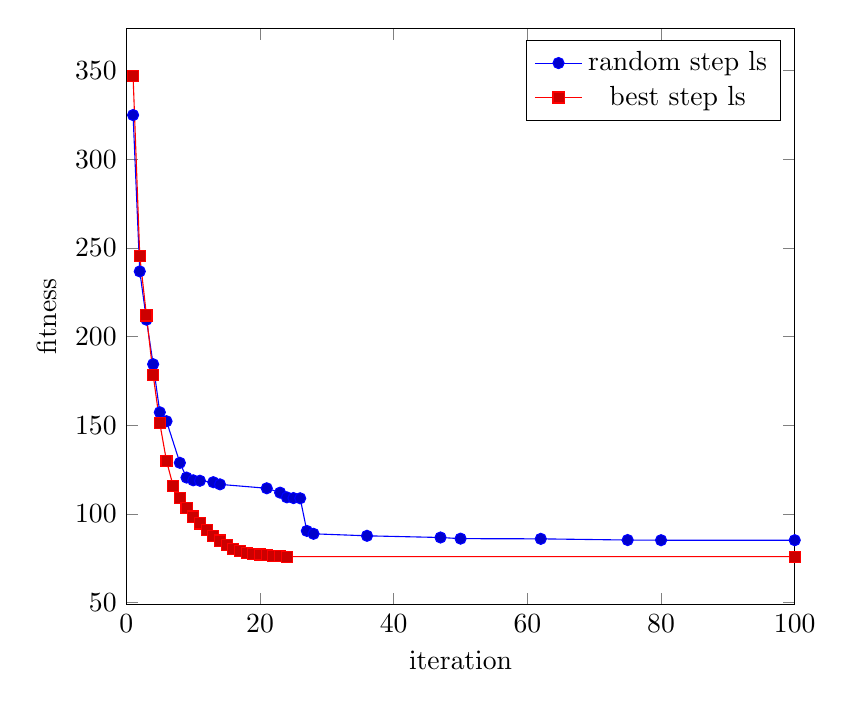
\begin{tikzpicture}
 \begin{axis}[
   width=0.7\textwidth,
   scale only axis,
   xlabel=iteration,
   ylabel=fitness,
   xmin=0,xmax=100,
   domain=0:100]
   \addplot coordinates {
     (0,inf)
     (1,324.942)
     (2,236.782)
     (3,209.541)
     (4,184.435)
     (5,157.321)
     (6,152.289)
     (8,128.823)
     (9,120.497)
     (10,118.965)
     (11,118.708)
     (13,117.899)
     (14,116.674)
     (21,114.465)
     (23,112.007)
     (24,109.374)
     (25,108.944)
     (26,108.819)
     (27,90.4234)
     (28,88.7929)
     (36,87.6585)
     (47,86.7098)
     (50,86.0617)
     (62,85.9504)
     (75,85.279)
     (80,85.1812)
     (100,85.1812)
   };
   \addlegendentry{random step ls}
   \addplot coordinates {
     (0,inf)
     (1,346.828)
     (2,245.422)
     (3,211.931)
     (4,178.561)
     (5,151.073)
     (6,129.859)
     (7,115.752)
     (8,108.788)
     (9,103.321)
     (10,98.5095)
     (11,94.646)
     (12,90.7951)
     (13,87.4437)
     (14,84.9935)
     (15,82.5473)
     (16,80.3739)
     (17,78.9966)
     (18,78.1543)
     (19,77.4955)
     (20,77.1273)
     (21,76.7786)
     (22,76.46)
     (23,76.0552)
     (24,75.926)
     (100,75.926)
   };
   \addlegendentry{best step ls}
 \end{axis}
 \end{tikzpicture}
\end{figure}

\end{figure}
\begin{figure}
\pgfsetplotmarksize{0pt}
\begin{figure}
 \centering
 \caption{\label{fl_conv6}UflLib/Euclid/1011EuclS.txt},
 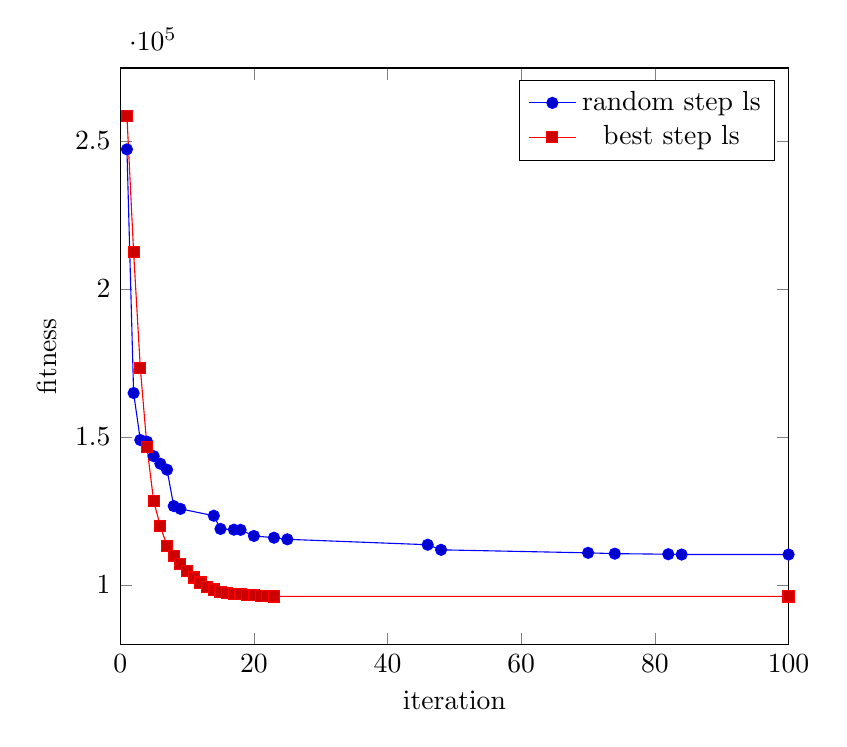
\begin{tikzpicture}
 \begin{axis}[
   width=0.7\textwidth,
   scale only axis,
   xlabel=iteration,
   ylabel=fitness,
   xmin=0,xmax=100,
   domain=0:100]
   \addplot coordinates {
     (0,inf)
     (1,247173)
     (2,164855)
     (3,148983)
     (4,148438)
     (5,143524)
     (6,140956)
     (7,138947)
     (8,126665)
     (9,125722)
     (14,123396)
     (15,118937)
     (17,118697)
     (18,118633)
     (20,116575)
     (23,115980)
     (25,115436)
     (46,113604)
     (48,111881)
     (70,110862)
     (74,110592)
     (82,110399)
     (84,110288)
     (100,110288)
   };
   \addlegendentry{random step ls}
   \addplot coordinates {
     (0,inf)
     (1,258418)
     (2,212384)
     (3,173393)
     (4,146526)
     (5,128358)
     (6,119830)
     (7,113211)
     (8,109737)
     (9,107133)
     (10,104709)
     (11,102534)
     (12,100826)
     (13,99429)
     (14,98453)
     (15,97721)
     (16,97269)
     (17,96972)
     (18,96841)
     (19,96724)
     (20,96670)
     (21,96416)
     (22,96355)
     (23,96135)
     (100,96135)
   };
   \addlegendentry{best step ls}
 \end{axis}
 \end{tikzpicture}
\end{figure}

\end{figure}

\begin{figure}[ht]
  \begin{tabular}[ht]{|l||c|c|c|c|c|c|H}
\cline{1-7}
 & 2511EuclS & 1811EuclS & 1211EuclS & 111EuclS & 1911EuclS & 2711EuclS & \\ \cline{1-7}\cline{1-7} 
optimum &99195 & 100189 & 98528 & 96116 & 98617 & 93845 & \\ \cline{1-7}
local search &1.0023 & 1.0165 & 1 & 1.01472 & 1.00671 & 1.00498 & \\ \cline{1-7}
ls fast &1.00605 & 1 & 1 & 1.00744 & 1.01128 & 1 & \\ \cline{1-7}
3 apx &1.19845 & 1.10865 & 1.23954 & 1.09184 & 1.10833 & 1.13838 & \\ \cline{1-7}
random &1.13476 & 1.12494 & 1.12943 & 1.1231 & 1.12784 & 1.11763 & \\ \cline{1-7}
\end{tabular}
\end{figure}

\subsection{MCTS}

Columns are titled in format $<test\_name>$ / $<samples\_multiplayer>$.

\begin{figure}[ht]
  \begin{tabular}[ht]{|l||c|c|c|c|H}
\cline{1-5}
 & 1011EuclS, sampling 10 & 1011EuclS, sampling 20 & 1011EuclS, sampling 50 & 1011EuclS, sampling 100 & \\ \cline{1-5}\cline{1-5} 
Optimal &95868 & 95868 & 95868 & 95868 & \\ \cline{1-5}
PolicyRandMean &98905 & 99303 & 98273 & 98034 & \\ \cline{1-5}
PolicyEpsMean &103719 & 102732 & 103541 & 100475 & \\ \cline{1-5}
PolicyEpsBest &110548 & 110198 & 109415 & 101247 & \\ \cline{1-5}
PolicyMuSigma &120849 & 111799 & 127288 & 123153 & \\ \cline{1-5}
\end{tabular}
\end{figure}

\begin{figure}[ht]
  \begin{tabular}[ht]{|l||c|c|c|c|H}
\cline{1-5}
 & 1111EuclS / 10 & 1111EuclS / 20 & 1111EuclS / 50 & 1111EuclS / 100 & \\ \cline{1-5}\cline{1-5} 
Optimal &97181 & 97181 & 97181 & 97181 & \\ \cline{1-5}
PolicyRandMean &101215 & 99235 & 101672 & 100083 & \\ \cline{1-5}
PolicyEpsMean &102671 & 101552 & 103163 & 104446 & \\ \cline{1-5}
PolicyEpsBest &104017 & 111955 & 114720 & 104598 & \\ \cline{1-5}
PolicyMuSigma &123367 & 121102 & 124145 & 117391 & \\ \cline{1-5}
\end{tabular}

\end{figure}

\begin{figure}[ht]
  \begin{tabular}[ht]{|l||c|c|c|c|H}
\cline{1-5}
 & 2211EuclS, sampling 10 & 2211EuclS, sampling 20 & 2211EuclS, sampling 50 & 2211EuclS, sampling 100 & \\ \cline{1-5}\cline{1-5} 
Optimal &98238 & 98238 & 98238 & 98238 & \\ \cline{1-5}
PolicyRandMean &101815 & 101938 & 101645 & 102111 & \\ \cline{1-5}
PolicyEpsMean &104751 & 103619 & 104756 & 103999 & \\ \cline{1-5}
PolicyEpsBest &108500 & 113070 & 106297 & 110863 & \\ \cline{1-5}
PolicyMuSigma &124487 & 120372 & 117375 & 118530 & \\ \cline{1-5}
\end{tabular}
\end{figure}

As we can see raising $samples\_multiplayer$ doesn't improve quality of answer too much,
on the other hand increasing $samples\_multiplayer$ by a factor of $k$ increases the
running time by the same factor.
